\chapter{Calculation Objects} \label{Ch:CalculationObjects}

GMAT has the ability to calculate numerous quantities that are
dependent upon the states of objects, coordinate systems, and the
mission sequence.   These calculation objects can range from the
spacecraft state, to the local atmospheric density, to the
positions of celestial bodies with respect to spacecraft, or other
celestial bodies.  In chapter, we present how GMAT performs these
calculations by showing the mathematical algorithms.

The chapter begins by discussing different orbit state
representations.  Each of the orbit state representations
available in GMAT are defined.  Next we present the algorithms
used to convert between different state representations.  These
include the Keplerian elements, modified Keplerian elements,
Cartesian state, spherical state, and the equinoctial elements. In
the second section we present how GMAT calculates all calculation
parameters. Examples include the orbit period, percent shadow, and
energy. The algorithms to calculate all parameters are included
and described in detail. We conclude this chapter with a
presentation of the algorithms used to calculate libration point
and barycenter locations.

\section{Spacecraft State Representations} \index{Orbit state
representations}

There are several state representations that can be used in GMAT
to define the state of a spacecraft object.  These include the
Keplerian elements, Cartesian state, equinoctial elements,
spherical elements, and the modified Keplerian elements.  In the
following subsections, we discuss the definitions of these states
types, and show how GMAT converts between the different state
representations.

\subsection{Definitions}

The Keplerian elements are one of the most commonly used state
representations.  They provide a way to define the spacecraft
state in way that provides an intuitive understanding of the
motion of spacecraft in orbit.  The Keplerian elements are denoted
$a$, $e$, $i$, $\omega$, $\Omega$, and $\nu$. They are defined in
detail in Table \ref{Table:KeplerianElements} and illustrated in
Fig. \ref{fig:KeplerianElements}.  Sections \ref{Sec:Cart2Kep} and
\ref{Sec:Kep2Cart} show the algorithms that GMAT uses to convert
between the Keplerian elements and the cartesian state.
\index{Keplerian elements!definition}
%

\begin{figure*}[htb]
\index{Keplerian elements} \centerline{
\begin{picture}(100,545)
\special{psfile=Images/OrbitElements.eps hoffset= -195 voffset= 75
hscale=80
vscale=80}\makebox(-78,600){$\hat{\mathbf{x}}_I$,$\Upsilon$}
\makebox(40,610){$\hat{\mathbf{x}}_{ep}$} \makebox(10,685){$\Omega$}
\makebox(215,795){$\omega$} \makebox(-120,840){$y_I$}
\makebox(-135,968){$\mathbf{x}_p$}\makebox(-255,980){$\nu$}
\makebox(-485,1083){$z_I$} \makebox(-540,1028){$i$}
    \makebox(-610,1060){$\mathbf{h}$, $\hat{\mathbf{z}}_{ep}$}
    \makebox(-340,610){$\mathbf{N}$}
\end{picture}}\vskip -3.95 in  \caption{ The Keplerian Elements } \label{fig:KeplerianElements}
\end{figure*}

The cartesian state is another common state representation and is
often used in the numerical integration of the equations of
motion.  The cartesian state with respect to a given coordinate
system is described in detail in Table
\ref{Table:CartesianStates}. \index{Cartesian state!definition}


The equinoctial elements are a set of non-singular elements that
can be used to describe the state of a spacecraft.  Because they
are nonsingular, they are useful for expressing the equations of
motion in Variation of Parameters (VOP) form.  The elements can be
unintuitive to use however.  The equinoctial elements are
described in detail in Table \ref{Table:EquinoctialElements}.
%

\begin{figure*}[htb]
\index{Spherical elements} \centerline{
\begin{picture}(100,420)
\special{psfile=Images/SphericalElements.eps hoffset= -100 voffset=
75
hscale=55 vscale=55} \makebox(-280,360){$\mathbf{x}$}%
\makebox(140,590){$\mathbf{y}$}%
\makebox(-435,820){$\mathbf{z}$}%
\makebox(-410,530){$\lambda$}%
\makebox(-273,636){$\delta$}%
\makebox(-330,695){$\mathbf{r}$}%
\makebox(-250,770){$\mathbf{v}$}%
\makebox(90,710){$\mathbf{v}$}%
\makebox(10,675){$\hat{\mathbf{r}}$}%
\makebox(-350,650){North}%
\makebox(-275,635){$\psi$}%
\makebox(-180,597){$\alpha_f$}%
\end{picture}}\vskip -2.5 in  \caption{ The Spherical Elements } \label{fig:SphericalElements}
\end{figure*}
%

The modified Keplerian elements are similar to the Keplerian
elements except $a$ and $e$ are replaced with the radius of
periapsis $r_p$, and the radius of apoapsis $r_a$. $r_p$ and $r_a$
are often more convenient and intuitive for describing the
dimensions of a Keplerian orbit than $a$ and $e$.  The modified
Keplerian elements are defined in detail in Table
\ref{Table:ModKeplerianElements}. Note that both the Keplerian and
modified Keplerian elements are undefined for parabolic orbits
because the semimajor axis is infinite.  Currently, GMAT does not
support parabolic orbits for this reason.  Let's begin by looking
at how GMAT converts from the Cartesian state to the Keplerian
elements.

\index{Modified Keplerian elements!definition}
%

\subsection{Cartesian State to Keplerian Elements}\label{Sec:Cart2Kep}  \index{Cartesian state!to
Keplerian} \index{Keplerian elements!from cartesian}

The conversion from the Cartesian state to the Keplerian elements
has four special cases:  elliptic inclined, circular inclined,
elliptic equatorial, and circular equatorial.  Certain orbital
elements are undefined for some of the cases.  For example, the
right ascension of the ascending node, $\Omega$, is undefined for
equatorial orbits.  However, computer systems don't handle
undefined values gracefully.  In this section, we'll see how the
orbital elements are defined for each of the special cases, and
how GMAT calculates the orbital elements for each case.

%
\begin{table*} \caption{The Cartesian State}
\centering \index{Cartesian state!definition}
\begin{tabular}{p{.5 in} p{2.0 in}}
  \hline\hline
  % after \\: \hline or \cline{col1-col2} \cline{col3-col4} ...
   Symbol &  Description \\
  \hline
  $x$ &  $x$-component of position\\
%
  $y$ &  $y$-component of position \\
  %
  $z$ &  $z$-component of position \\
  %
  $\dot{x}$ &  $x$-component of velocity\\
  %
  $\dot{y}$ & $y$-component of velocity\\
  %
  $\dot{z}$ & $z$-component of velocity \\
  \hline\hline \label{Table:CartesianStates}
\end{tabular}
\end{table*}

\begin{table*} \caption{The Keplerian Elements (also see Fig. \ref{fig:KeplerianElements})}
\centering \index{Keplerian elements!definition}
\begin{tabular}{p{.5 in} p{1.5 in} p{3.5 in}}
  \hline\hline
  % after \\: \hline or \cline{col1-col2} \cline{col3-col4} ...
   Symbol & Name & Description \\
  \hline
  $a$ & semimajor axis & The semimajor contains information on the type and size of an orbit.
  If $a>0$ the orbit is elliptic.  If $a < 0$ the orbit is hyperbolic. $a = \infty$ for parabolic orbits. \\
 %
  $e$ & eccentricity & The eccentricity contains information on the shape of an orbit.  If $e = 0$, then the orbit is circular. If $0 < e < 1$ the orbit is
  elliptical.  If $e = 1$ the orbit is parabolic.  If $e > 1$ then the orbit is hyperbolic. \\
  %
  $i$ & inclination & The inclination is the angle between the $\hat{\mathbf{z}}_I$ axis and the orbit normal direction $\mathbf{h}$.  If $i \leq 90^{\circ}$ then the orbit is prograde.
  If $i > 90^{\circ}$ then the orbit is retrograde.  \\
  %
  $\omega$ & argument of periapsis & The argument of periapsis is the angle between a vector pointing at periapsis  and a vector pointing in the direction of the line of nodes. The argument of periapsis is undefined for circular orbits.\\
  %
  $\Omega$ & right ascension of  the ascending node& $\Omega$ is defined as the angle between $\hat{\mathbf{x}}_I$ and $\mathbf{N}$ measured
  counterclockwise.
    $\mathbf{N}$ is defined as the vector pointing from the center of the central body to the spacecraft, when the spacecraft crosses the bodies equatorial plane
  from the southern to the northern hemisphere.  $\Omega$ is undefined for equatorial orbits.   \\
  %
  $\nu$ & true anomaly & The true anomaly is defined as the angle between a vector pointing at periapsis and a vector pointing at the spacecraft.
  The true anomaly is undefined for circular orbits. \\
  \hline\hline \label{Table:KeplerianElements}
\end{tabular}
\end{table*}

%
\begin{table*} \caption{Keplerian Elements for Special Cases}
 \centering \index{Keplerian elements!special cases}
\begin{tabular}{p{1.25 in} p{1.35 in} p{3.2 in}  }
  \hline\hline
  % after \\: \hline or \cline{col1-col2} \cline{col3-col4} ...
   Orbit Type & Numerical Threshold & Description \\
  \hline \\
  %--------------
  Elliptic Inclined & $e \geq 10^{-11}$, $i \geq 10^{-11}$ & $\Omega$ is the angle between the $x$-axis and the line of nodes. $\omega$ is the angle between the line of nodes and the eccentricity vector, $\nu$ is
                                                     the angle between the eccentricity vector and the spacecraft position vector.\\
  %--------------
  Elliptic Equatorial & $e \geq 10^{-11}$, $i < 10^{-11}$ & $\Omega = 0$, $\omega$ is the angle between the $x$-axis and the eccentricity vector, $\nu$ is
                                                     the angle between the eccentricity vector and the spacecraft position vector.\\
  %--------------
  Circular Inclined & $e < 10^{-11}$, $i \geq 10^{-11}$  & $\Omega$ is the angle between the $x$-axis and the line of nodes, $\omega = 0$, $\nu$ is
                                                     the angle between the line of nodes and the spacecraft position vector.\\
  %--------------
  Circular Equatorial & $e < 10^{-11}$, $i < 10^{-11}$ & $\Omega = 0$, $\omega = 0$, $\nu$ is the angle between the $x$-axis and the spacecraft position vector. \\
  \hline\hline \label{Table:KeplerianElementsSpecialCases}
\end{tabular}
\end{table*}

\noindent Given:  $\mathbf{r}$, $\mathbf{v}$, and $\mu$\\

\noindent Find: $a$, $e$, $i$, $\omega$, $\Omega$, and $\nu$

We begin by calculating the specific angular momentum and its
magnitude.
%
\begin{equation}
     \mathbf{h} = \mathbf{r} \times \mathbf{v}
\end{equation}
%
\begin{equation}
     h = \|\mathbf{h} \|
\end{equation}
%
A vector pointing in the direction of the line of nodes is
%
\begin{equation}
     \mathbf{n} = [ \hspace{0.05 in} 0 \hspace{0.1 in} 0 \hspace{0.1 in} 1 \hspace{0.05
     in}]^T \times \mathbf{h}
\end{equation}
%
\begin{equation}
     n = \| n\|
\end{equation}
%
The orbit eccentricity and energy are calculated using
%
\begin{equation}
    r = \| \mathbf{r} \|
\end{equation}
%
\begin{equation}
    v = \| \mathbf{v} \|
\end{equation}
%
\begin{equation}
     \mathbf{e} = \displaystyle\frac{(v^2 - \displaystyle\frac{\mu}{r} )\mathbf{r} - (\mathbf{r}\cdot\mathbf{v}  )\mathbf{v}}{\mu}
\end{equation}
%
\begin{equation}
     e = \| \mathbf{e} \|
\end{equation}
%
\begin{equation}
     \xi = \frac{v^2}{2} - \frac{\mu}{r}
\end{equation}
%

Recall that for parabolic orbits, the semimajor axis is infinite
and the energy is zero. GMAT checks to see if the orbit is near
parabolic and returns an error message in this case.
The following error check avoids the possibility of a divide by zero:\\

\noindent if $|1 - e|> 10^{-30}$, then
\begin{equation}
     a = -\frac{\mu}{2\xi}
\end{equation}
%
otherwise, report  error and return.  The error reported is:
``Warning: GMAT does not support parabolic orbits in conversion
from cartesian to Keplerian state".

If the orbit is not parabolic according to the above definition,
then we continue and calculate the inclination.
%
\begin{equation}
     i = \cos^{-1}\left(\frac{h_z}{h}\right)
\end{equation}

There are four special cases for $\Omega$, $\omega$, and $\nu$ and
each case is treated differently.

\noindent\textit{Special Case 1:  Non-circular, Inclined Orbit  }

\noindent if $(e \geq 10^{-11})$  and $(i \geq 10^{-11})$, then
%
\begin{equation}
    \Omega = \cos^{-1}\left(\frac{n_x}{n}\right)
\end{equation}
%
Fix quadrant for $\Omega$: if $n_y < 0$, then $\Omega = 2\pi -
\Omega$
%
\begin{equation}
    \omega = \cos^{-1}\left( \frac{\mathbf{n}\cdot\mathbf{e}}{ne}\right)
\end{equation}
%
Fix quadrant for $\omega $:  if $e_z < 0$, then $\omega = 2\pi -
\omega$
%
\begin{equation}
    \nu = \cos^{-1}\left( \frac{\mathbf{e}\cdot\mathbf{r}}{er}\right)
\end{equation}
%
Fix quadrant for $\nu $:  if $\mathbf{r} \cdot \mathbf{v} < 0$, then
$\nu = 2\pi - \nu$

\noindent\textit{Special Case 2:  Non-circular, Equatorial Orbit
}

\noindent if $(e \geq 10^{-11})$  and $(i < 10^{-11})$, then
%
\begin{equation}
    \Omega = 0
\end{equation}
%
\begin{equation}
     \omega = \cos^{-1}{\frac{e_x}{e}}
\end{equation}
%
Fix quadrant for $\omega $: if $e_y < 0$, then $\omega = 2\pi -
\omega$
%
\begin{equation}
    \nu = \cos^{-1}\left( \frac{\mathbf{e}\cdot\mathbf{r}}{er}\right)
\end{equation}
%
Fix quadrant for $\nu $:  if $\mathbf{r} \cdot \mathbf{v} < 0$, then
$\nu = 2\pi - \nu$
%

\noindent\textit{Special Case 3:  Circular, Inclined Orbit  }

\noindent if $(e < 10^{-11})$  and $(i \geq 10^{-11})$, then
%
\begin{equation}
    \Omega = \cos^{-1}\left(\frac{n_x}{n}\right)
\end{equation}
%
Fix quadrant for $\Omega$: if $n_y < 0$, then $\Omega = 2\pi -
\Omega$
\begin{equation}
     \omega = 0
\end{equation}
%
\begin{equation}
    \nu = \cos^{-1}\left( \frac{\mathbf{n}\cdot\mathbf{r}}{nr}\right)
\end{equation}
%
Fix quadrant for $\nu$:  if $r_z < 0$, then $\nu = 2\pi - \nu$

\noindent\textit{Special Case 4:  Circular, Equatorial Orbit  }

\noindent if $(e < 10^{-11})$  and $(i < 10^{-11})$, then
%
\begin{equation}
     \Omega = 0
\end{equation}
%
\begin{equation}
     \omega = 0
\end{equation}
%
\begin{equation}
    \nu = \cos^{-1}\left( \frac{r_x}{r}\right)
\end{equation}
%
Fix quadrant for $\nu$:  if $r_y < 0$, then $\nu = 2\pi - \nu$
%

In the next section, we look at how to perform the inverse
transformation and convert from Keplerian elements to the
Cartesian state vector.

\subsection{Keplerian Elements to Cartesian \\ State}


\label{Sec:Kep2Cart} \index{Keplerian elements!to
cartesian} \index{Cartesian state!from Keplerian}

The transformation from the Keplerian elements to the cartesian
state is one of the most common state transformations in
astrodynamics.  We previously defined both state types and refer
you to Tables \ref{Table:CartesianStates} and
\ref{Table:KeplerianElements} for their definitions.  Below we
show the algorithm that GMAT uses to convert from the Keplerian
elements to the Cartesian state.

\noindent Give:  $a$, $e$, $i$, $\Omega$, $\omega$, $\nu$, and
$\mu$

\noindent Find:  $\mathbf{r}$  and $\mathbf{v}$

We begin by checking that the magnitude of the position vector is
not infinite.  This avoids the possibility of a division by zero.

\noindent if ($1+e\cos{\nu}$ $<$ 1e-30), then display error and
return: ``Warning: Radius is near infinite in keplerian to
cartesian conversion"

\noindent If their is not a divide by zero issue we continue  by
calculating the semilatus rectum, and the radius.
%
\begin{equation}
    p = a(1-e^2);
\end{equation}
%
\begin{equation}
     r = \frac{p}{1+e\cos{\nu}}
\end{equation}
%
The position components of the cartesian state vector are
calculated using the following three equations.
%
\begin{equation}
     x = r\left(\cos{(\omega + \nu)}\cos{\Omega} - \cos{i}\sin{(\omega + \nu)}\sin{\Omega}\right)
\end{equation}
\begin{equation}
     y = r\left(\cos{(\omega + \nu)}\sin{\Omega} + \cos{i}\sin{(\omega + \nu)}\cos{\Omega}\right)
\end{equation}
\begin{equation}
     z = r\left(\sin{(\omega + \nu)}\sin{i}\right)
\end{equation}
%

Before calculating the velocity components we check to ensure the
orbit is not parabolic.  This avoids another possible division by
zero.

\noindent if ($\| p\| < 1e-30$), then error and return: ``Warning:
GMAT does not support parabolic orbits in conversion from
keplerian to cartesian elements".

\noindent If the orbit is not parabolic, we continue and calculate
the velocity components using
%
\begin{equation}\begin{split}
     \dot{x} = \sqrt{\frac{\mu}{p}} &  \left( \cos{\nu} + e \right)
     \left( -\sin{\omega}\cos{\Omega} - \cos{i}\sin{\Omega}\cos{\omega}
     \right)- \\ &\sqrt{\frac{\mu}{p}}  \sin{\nu}\left(\cos{\omega}\cos{\Omega} - \cos{i}\sin{\Omega}\sin{\omega} \right)
      \end{split}
\end{equation}
%
\begin{equation}\begin{split}
     \dot{y} =    \sqrt{\frac{\mu}{p}}&  \left( \cos{\nu} + e \right)
     \left( -\sin{\omega}\sin{\Omega} + \cos{i}\cos{\Omega}\cos{\omega}
     \right)- \\\ & \sqrt{\frac{\mu}{p}}\sin{\nu}\left(\cos{\omega}\sin{\Omega} + \cos{i}\cos{\Omega}\sin{\omega} \right)
     \end{split}
\end{equation}
%
\begin{equation}
     \dot{z} = \sqrt{\frac{\mu}{p}} \left[ \left( \cos{\nu} + e \right)\sin{i}\cos{w} - \sin{\nu}\sin{i}\sin{\omega}      \right]
\end{equation}

Now let's look at how to calculate the cartesian state given the
equinoctial elements.

\subsection{Equinoctial Elements to Cartesian \\State}  \index{Equinoctial elements!to
cartesian}\index{Cartesian state!from Equinotial}
\label{Sec:EquinoctialtoCartesian}

The equinoctial elements used in GMAT are defined in Table
\ref{Table:EquinoctialElements}.  The algorithm to convert from
equinoctial elements to the cartesian state was taken from the
GTDS Mathematical Theory \cite{GTDS}.

\begin{table*} \caption{The Equinoctial Elements}
\centering \index{Equinoctial elements!definition}
\begin{tabular}{p{.5 in} p{5.0 in}}
  \hline\hline
  % after \\: \hline or \cline{col1-col2} \cline{col3-col4} ...
   Symbol &  Description \\
  \hline
  $a$ &  The semimajor contains information on the type and size of an orbit.  If $a>0$ the orbit is elliptic.  If $a < 0$ the orbit is hyperbolic. \\
%
  $h$ &  The projection of the eccentricity vector onto the $\hat{\mathbf{y}}_{ep}$ axis. \\
  %
  $k$ & The projection of the eccentricity vector onto the $\hat{\mathbf{x}}_{ep}$ axis. \\
  %
  $p$ &  The projection of $\mathbf{N}$  onto the $\hat{\mathbf{y}}_{ep}$ axis.\\
  %
  $q$ & The projection of $\mathbf{N}$  onto the $\hat{\mathbf{x}}_{ep}$ axis.  \\
  %
  $\lambda$ & The mean longitude. \\
  \hline\hline \label{Table:EquinoctialElements}
\end{tabular}
\end{table*}

\noindent Given: $a$, $h$, $k$, $p$, $q$, $\lambda$, and $\mu$

\noindent Find: $\mathbf{r}$ and $\mathbf{v}$

We begin by using the mean longitude, $\lambda$, to find the true
longitude $F$.  The equation relating the two is transcendental:
\begin{equation}
     \lambda = F + h\cos{F} - k \sin{F}
\end{equation}
%
We use the Newton-Raphson method to solve for $F$, using $\lambda$
as the initial guess.  We iterate on the following equation until
$|F(i+1) - F(i)| < 10^{-10}$.
%
\begin{equation}
    F(i+1) = F(i) - \frac{f(F)}{f'(F)}
\end{equation}
%
where
%
\begin{eqnarray}
    f(F) &=& F + h \cos(F) - k\sin(F) - \lambda \\
    %
    f'(F) &=& 1 - h \sin(F) - k \cos(F)
\end{eqnarray}

Once the true longitude is calculated, we continue with
%
\begin{equation}
   \beta = \frac{1}{1 + \sqrt{1 - h^2 - k^2}} \label{Eq:Beta}
\end{equation}
%
\begin{equation}
   n = \frac{mu}{a^3}
\end{equation}
%
\begin{equation}
   r = a(1 - k\cos{F} - h\sin{f})
\end{equation}

The cartesian components expressed in the equinoctial coordinate
system can be calculated using.
%
\begin{equation}
   X_1 = a\left[ ( 1 - h^2 \beta) \cos{F} + h k \beta \sin{F} - k   \right]
\end{equation}
%
\begin{equation}
   Y_1 = a\left[ ( 1 - k^2 \beta) \sin{F} + h k \beta \cos{F} - h   \right]
\end{equation}
%
\begin{equation}
  \dot{X}_1 = \frac{n a^2}{r}\left[h k \beta \cos{F} - (1 - h^2 \beta)\sin{F}   \right]
\end{equation}
%
\begin{equation}
  \dot{Y}_1 = \frac{n a^2}{r}\left[  (1 - k^2 \beta)\cos{F}  -  h k \beta \sin{F}   \right]
\end{equation}
%

The transformation from the equinoctial system to the inertial
Cartesian system is given by
%
\begin{equation}
   \mathbf{r} = X_1 \hat{\mathbf{f}} + Y_1 \hat{\mathbf{g}}
\end{equation}
%
\begin{equation}
   \mathbf{v} = \dot{X}_1 \hat{\mathbf{f}} + \dot{Y}_1 \hat{\mathbf{g}}
\end{equation}
%
where
%
\begin{equation}
    \left[ \hat{\mathbf{f}} \hspace{.1 in} \hat{\mathbf{g}} \hspace{.1 in} \hat{\mathbf{w}}
    \right]=  \frac{1}{1+p^2+q^2}\hspace{.1 in} \mathbf{Q}
\end{equation}
%
and
%
\begin{equation} \mathbf{Q} =
 \begin{pmatrix}
               1 - p^2 + q^2 &
               2 p q j &
               2 p \\
%
               2 p q&
               \left( 1 + p^2 - q^2 \right)j &
               -2 q \\
               %
               - 2 p j&
               2 q &
               \left(1 - p^2 - q^2  \right)j \\
               %
     \end{pmatrix}
\end{equation}
%
and
%
\noindent j = 1 for direct orbits ( $0\leq i \leq 90^{\circ}$ )\\
 j = -1 for retrograde orbits ( $90 < i \leq 180^{\circ}$ )\\

Now let's look at how to calculate the cartesian state given the
equinoctial elements.

\subsection{Cartesian State to Equinoctial \\ Elements}  \index{Equinoctial elements!from cartesian}
\index{Cartesian state!to Equinotial}
\label{Sec:CartesiantoEquinoctial}

The equinoctial elements used in GMAT are defined in Table
\ref{Table:EquinoctialElements}.  The algorithm to convert from
the cartesian state to the equinoctial elements was taken from the
GTDS Mathematical Theory \cite{GTDS}.

\noindent Given:  $\mathbf{r}$, $\mathbf{v}$, and $\mu$

\noindent Fine:  $a$, $h$, $k$, $p$, $q$, $\lambda$, and $\mu$

We begin by calculating the semimajor axis and the eccentricity
vector.
%
\begin{equation}
    r = \| \mathbf{r} \|
\end{equation}
%
\begin{equation}
    v = \| \mathbf{v} \|
\end{equation}
%
\begin{equation}
     a = \displaystyle\frac{1}{\displaystyle\frac{2}{r} - \displaystyle\frac{v^2}{\mu}}
\end{equation}
%
\begin{equation}
     \mathbf{e} = -\frac{ \mathbf{r} }{r} - \frac{\left( \mathbf{r} \times \mathbf{v} \right) \times \mathbf{v}}{\mu}
\end{equation}
%
The angular momentum vector is
%
\begin{equation}
   \hat{\mathbf{h}} = \frac{\mathbf{r} \times \mathbf{v} }{ \| \mathbf{r} \times \mathbf{v} \|}
\end{equation}
%
The unit vectors that define the equinoctial coordinate system can
be calculated using
%
\begin{equation}
   f_x = 1 - \frac{h_x^2}{ 1 + h_z^j}
\end{equation}
%
\begin{equation}
   f_y = -\frac{h_x h_y}{ 1 + h_z^j}
\end{equation}
%
\begin{equation}
   f_z = -h_x^j
\end{equation}
%
where $j$ is described in Section \ref{Sec:EquinoctialtoCartesian}.\\
%
\begin{equation}
    \hat{\mathbf{g}} = \hat{\mathbf{h}} \times \hat{\mathbf{f}}
\end{equation}
%

We now have the necessary information to calculate the elements
$h$, $k$, $p$, and $q$ using the following relationships.
%
\begin{equation}
    h = \mathbf{e} \cdot \hat{\mathbf{g}}
\end{equation}
%
\begin{equation}
    k = \mathbf{e} \cdot \hat{\mathbf{f}}
\end{equation}
%
\begin{equation}
    p = \frac{h_x}{1+h_z^j}
\end{equation}
%
\begin{equation}
    q = - \frac{h_y}{1+h_z^j}
\end{equation}
%

The final element to calculate is the mean longitude, $\lambda$.
We begin by computing the true longitude, $F$,  using
%
\begin{equation}
    X_1 = \mathbf{r} \cdot \hat{\mathbf{f}}
\end{equation}
%
\begin{equation}
    Y_1 = \mathbf{r} \cdot \hat{\mathbf{g}}
\end{equation}
%
and
%
\begin{equation}
     \cos{F} = k + \frac{ \left( 1 - k^2 \beta \right) X_1 - h k \beta Y_1}{a\sqrt{1 - h^2 - k^2}}
\end{equation}
%
\begin{equation}
     \sin{F} = h + \frac{ \left( 1 - h^2 \beta \right) Y_1 - h k \beta X_1}{a\sqrt{1 - h^2 - k^2}}
\end{equation}
%
\begin{equation}
     F = \tan^{-1}_2\left( \frac{\sin{F}}{\cos{F}}\right)
\end{equation}
%
where $\beta$ is given by Eq.~\ref{Eq:Beta}.  The mean longitude
is computed using the generalized Kepler equation
%
\begin{equation}
    \lambda = F + h \cos{f} - k \sin{F}
\end{equation}

Now let's look at transformations involving the spherical
elements.

\subsection{Cartesian State to SphericalAZFPA State}
\label{Sec:CarttoSphericalAZFPA} \index{Cartesian state!to
SphericalAZFPA} \index{SphericalAZFPA! from Cartesian state }

The spherical state, with azimuth, $\alpha_f$, and flight path
angle, $\psi$, is described in Table \ref{Table:SphericalElements}
and Fig. \ref{fig:SphericalElements}.  The algorithm below shows
how GMAT converts from the cartesian state to the spherical state
with azimuth and flight path angle.

\noindent Given:  $\mathbf{r}$ and $\mathbf{v}$

\noindent Find:  $r$, $\lambda$, $\delta$, $v$, $\psi$, and
$\alpha_f$

\begin{table*} \caption{The Spherical Elements}
\centering \index{Spherical elements!definition}
\begin{tabular}{p{.5 in} p{1.5 in} p{3.5 in}}
  \hline\hline
  % after \\: \hline or \cline{col1-col2} \cline{col3-col4} ...
   Symbol & Name & Description \\
  \hline
  $r$ & $r$ & Magnitude of the position vector, $\|\mathbf{r}\|$ \\
    %
  $\lambda$ & Right Ascension & The between the projection of $\mathbf{r}$ into the $x-y$ and the $x$-axis.  Measured counterclockwise.   \\
%
  $\delta$ & Declination & The angle between $\mathbf{r}$ and the $x-y$ plane measured in the plane formed by $\mathbf{r}$ and $\hat{\mathbf{z}}$ . \\

  %
  $v$ & $v$ & Magnitude of the velocity vector, $\|\mathbf{v}\|$ \\
  %
  $\psi$ & Vertical flight path angle & The angle measured from a plane normal to $\mathbf{r}$ to the velocity vector $\mathbf{v}$, measured in the plane formed by $\mathbf{r}$  and $\mathbf{v}$   \\
  %
  $\alpha_f$ & Flight path azimuth & The angle measured from vector perpendicular  $\mathbf{r}$ and pointing north, to the projection of $\mathbf{v}$ into a plane normal to $\mathbf{r}$. \\
  \hline\hline \label{Table:SphericalElements}
\end{tabular}
\end{table*}

We begin by calculating the right ascension $\lambda$, and the
declination $\delta$.
%
\begin{equation}
    r = \| \mathbf{r} \| \label{Eq:Sphericalr}
\end{equation}
%
\begin{equation}
    \lambda= \tan^{-1}_2(y,x) \label{Eq:Sphericallambda}
\end{equation}
%
\begin{equation}
    \delta = \sin^{-1}(\frac{z}{r}) \label{Eq:Sphericaldelta}
\end{equation}
%
The magnitude of the velocity vector is simply
%
\begin{equation}
    v = \| \mathbf{v} \|  \label{Eq:Sphericalv}
\end{equation}
%
We calculate the vertical flight path angle, $psi$, using
%
\begin{equation}
    \psi = \cos^{-1}\left(  \frac{\mathbf{r} \cdot \mathbf{v} }{r v} \right)
\end{equation}
%
To calculate the azimuth angle, $\alpha_z$, we begin by
calculating the rotation matrix from the frame in which the
cartesian state is expressed in, $\mathcal{F}_{i}$, to a local
frame, $\mathcal{F}_{\ell}$, where $\hat{\mathbf{z}}$ is a unit
vector that points north.  The basis vectors of
$\mathcal{F}_{\ell}$ expressed in $\mathcal{F}_{i}$ can be
calculated using
%
\begin{equation}
    \hat{\mathbf{x}} =
    \begin{pmatrix}
        \cos(\delta)\cos(\lambda)\\
         \cos(\delta)\sin(\lambda)\\
          \sin(\delta)
    \end{pmatrix} \label{Eq:SphericalAZFPAx}
\end{equation}
%
\begin{equation}
    \hat{\mathbf{y}} =
    \begin{pmatrix}
          \cos(\lambda + \pi/2)\\
          \sin(\lambda + \pi/2)\\
          0
    \end{pmatrix}  \label{Eq:SphericalAZFPAy}
\end{equation}
%
\begin{equation}
    \hat{\mathbf{z}} =
    \begin{pmatrix}
          -\sin(\delta)\cos(\lambda)\\
          -\sin(\delta)\sin(\lambda)\\
          \cos(\delta)
    \end{pmatrix}  \label{Eq:SphericalAZFPAz}
\end{equation}
%
We can write the tranformation matrix that goes from
$\mathcal{F}_{i}$ to $\mathcal{F}_{\ell}$, $\mathbf{R}_{\ell i}$,
as
%
\begin{equation}
    \mathbf{R}_{\ell i} = [\hspace{.05 in} \hat{\mathbf{x}} \hspace{.1 in}
    \hat{\mathbf{y}} \hspace{.1in} \hat{\mathbf{z}} \hspace{.05 in}]^T
\end{equation}
%
The velocity in the local frame,  $\mathbf{v}'$, can be written as
%
\begin{equation}
    \mathbf{v}' = \mathbf{R}_{\ell i}\mathbf{v}
\end{equation}
%
Finally, we calculate the azimuth angle using
\begin{equation}
     \alpha_f = \tan^{-1}_2( v'_y, v'_z )
\end{equation}

Now that we have looked at how to convert from the Cartesian state
to the spherical state, let's look at the inverse transformation
that converts from the spherical state (with $\psi$ and
$\alpha_f$) to the cartesian state.

\subsection{SphericalAZFPA State to Cartesian State} \index{Cartesian
state!from SphericalAZFPA} \index{SphericalAZFPA! to Cartesian
state } \label{Sec:SphericalAZFPAtoCartesian}

In this section we present the algorithm used to convert from the
spherical state (with $\psi$ and $\alpha_f$) to the cartesian
state.

\noindent Given: $r$, $\lambda$, $\delta$, $v$, $\psi$, and
$\alpha_f$

\noindent Find:  $\mathbf{r}$ and $\mathbf{v}$

The components of the position vector are calculated using
%
\begin{eqnarray}
     x &=& r\cos{\delta} \cos{ \lambda } \label{Eq:Sphericalx}\\
     %
     y &=& r\cos{\delta}\sin{\lambda}  \label{Eq:Sphericaly}\\
     %
     z &=& r\sin{\delta} \label{Eq:Sphericalz}
\end{eqnarray}
%

We can write the velocity vector in terms of $v$, $\psi$, and
$\alpha_f$ as,
%
\begin{equation}
     \mathbf{v} = v\left[\cos( \psi )\hat{\mathbf{x}} + \sin( \psi )\sin(\alpha_f)\hat{\mathbf{y}} +
     \sin( \psi )\cos(\alpha_f)\hat{\mathbf{z}}\right]
     \label{Eq:SphericalAZFPAv}
\end{equation}
%
where, $\hat{\mathbf{x}}$, $\hat{\mathbf{y}}$, and
$\hat{\mathbf{x}}$ are given in Eqs.~(\ref{Eq:SphericalAZFPAx}),
(\ref{Eq:SphericalAZFPAy}), and (\ref{Eq:SphericalAZFPAz})
respectively.  Breaking down Eq.~(\ref{Eq:SphericalAZFPAv}) into
components gives us
%
\begin{equation}
\begin{split}
      v_x = v[ \cos{\psi}\cos{\delta}\cos{\lambda}- &\sin{\psi}(\sin{\alpha_f}\sin{\lambda}
       \\
      +  &\cos{\alpha_f}\sin{\delta}\cos{\lambda})]
\end{split}
\end{equation}
%
\begin{equation}
\begin{split}
      v_y = v[
      \cos{\psi}\cos{\delta}\sin{\lambda}+&\sin{\psi}(\sin{\alpha_f}\cos{\lambda}
      \\
      -&\cos{\alpha_f}\sin{\delta}\sin{\lambda})]
\end{split}
\end{equation}
%
\begin{equation}
      v_z = v[\cos{\psi}\sin{\delta}+\sin{\psi}\cos{\alpha_f}cos{\delta}]
\end{equation}
%

\subsection{Cartesian State to SphericalRADEC State}\index{Cartesian state! to
SphericalRADEC} \index{SphericalRADEC! from Cartesian State }

The conversion form the Cartesian state to the spherical state
with right ascension of velocity, $\lambda_v$, and declination of
velocity, $\delta_v$, is very similar to the transformation shown
in Sec. \ref{Sec:CarttoSphericalAZFPA}.  The algorithm to
calculate $\lambda_v$ and $\delta_v$ is shown below.

\noindent Given:  $\mathbf{r}$ and $\mathbf{v}$

\noindent Find:  $r$, $\lambda$, $\delta$, $v$, $\lambda_v$, and
$\delta_v$

To calculate $r$, $\lambda$, $\delta$, and $v$ we use
Eqs.~(\ref{Eq:Sphericalr}), (\ref{Eq:Sphericallambda}),
(\ref{Eq:Sphericaldelta}), and (\ref{Eq:Sphericalv}) respectively.
The right ascension of velocity, $\lambda_v$, and declination of
velocity, $\delta_v$, are calculated using
%
\begin{equation}
    \lambda_v= \tan^{-1}_2(v_y,v_x) \label{Eq:Sphericallambdav}
\end{equation}
%
\begin{equation}
    \delta_v = \sin^{-1}(\frac{v_z}{v}) \label{Eq:Sphericaldeltav}
\end{equation}
%

In the next section, we show the the transformation from the
spherical state  with right ascension of velocity, $\lambda_v$,
and declination of velocity, $\delta_v$, to the cartesian state.

\subsection{SphericalRADEC State to Cartesian State} \index{Cartesian state!from SphericalRADEC }

This transformation is similar to the conversion presented in Sec
\ref{Sec:SphericalAZFPAtoCartesian}.  The primary difference is
how the velocity is represented.

\noindent Given:  $r$, $\lambda$, $\delta$, $v$, $\lambda_v$, and
$\delta_v$

\noindent Find:  $\mathbf{r}$ and $\mathbf{v}$

The position components are calculated using Eqs.
(\ref{Eq:Sphericalx}), (\ref{Eq:Sphericaly}), and
(\ref{Eq:Sphericalz}).  The velocity components are calculated
using
%
\begin{eqnarray}
    v_x &=& v\cos{\lambda}\cos{\delta}\\
    v_y &=& v_x\tan{\lambda}\\
    v_z &=& v\sin{\delta}
\end{eqnarray}

In the last few subsections, we have looked at transformations
involving the spherical elements.  Now let's look at
transformations involving the modified Keplerian elements.

\subsection{Keplerian or Cartesian, to Modified Keplerian Elements} \index{Modified Keplerian elements!from Keplerian} \index{Keplerian elements!to modified Keplerian}

The modified Keplerian elements, described in Table
\ref{Table:ModKeplerianElements}, are similar to the classical
Keplerian elements.  The modified Keplerian elements use the
radius of apoapsis, $r_a$, and the radius of periapsis, $r_p$, to
describe the size and shape of an orbit.  The remaining elements,
$i$, $\Omega$, $\omega$, and $\nu$, are the same for both the
Keplerian and modified Keplerian elements. The modified Keplerian
elements, like the Keplerian elements, are undefined for parabolic
orbits.  Let's look at how GMAT calculates the modified


\begin{table*} \caption{The Modified Keplerian Elements}
\centering\index{Modified Keplerian elements!definition}
\begin{tabular}{p{.5 in} p{1.5 in} p{3.5 in}}
  \hline\hline
  % after \\: \hline or \cline{col1-col2} \cline{col3-col4} ...
   Symbol & Name & Description \\
  \hline
  $r_p$ & radius of periapsis & The radius of periapsis is the radius at the spacecrafts closest approach to the central body.  The radius of periapsis must be greater than zero, parabolic orbits are not currently supported. \\
%
  $r_a$ & radius of apoapsis  &  For an elliptic orbit $r_a$ is the radius at the spacecrafts farthest distance from the central body and $r_a>r_p$.  For hyperbolic orbits, $r_a<r_p$ and $r_a < 0 $  \\
  %
  $i$ & inclination & The inclination is the angle between the $\hat{\mathbf{z}}_I$ axis and the orbit normal direction $\mathbf{h}$.  If $i \leq 90^{\circ}$ then the orbit is prograde.
  If $i > 90^{\circ}$ then the orbit is retrograde.  \\
  %
  $\omega$ & argument of periapsis & The argument of periapsis is the angle between a vector pointing at periapsis,
  $\mathbf{x}_p$, and a vector pointing at the spacecraft. The argument of periapsis is undefined for circular orbits.\\
  %
  $\Omega$ & right ascension of  the ascending node& $\Omega$ is defined as the angle between $\hat{\mathbf{x}}_I$ and $\mathbf{N}$ measured
  counterclockwise.
    $\mathbf{N}$ is defined as the vector pointing from the center of the central body to the spacecraft, when the spacecraft crosses the bodies equatorial plane
  from the southern to the northern hemisphere.  $\Omega$ is undefined for equatorial orbits.   \\
  %
  $\nu$ & true anomaly & The true anomaly is defined as the angle between a vector pointing at periapsis, $\mathbf{x}_p$, and a vector pointing at the spacecraft.
  The true anomaly is undefined for circular orbits. \\
  \hline\hline \label{Table:ModKeplerianElements}
\end{tabular}
\end{table*}


\noindent Given:  $a$, $e$, $i$, $\omega$, $\Omega$, and $\nu$, or
$\mathbf{r}$, $\mathbf{v}$, and $\mu$

\noindent Find:  $r_p$ and $r_a$

If we are given the Cartesian state, we first calculate the
orbital elements using the algorithm in Sec. \ref{Sec:Kep2Cart}.
Knowing the Keplerian elements, we calculate $r_a$ and $r_p$ using
%
\begin{equation}
     r_a = a(1+e)
\end{equation}
%
\begin{equation}
     r_p = a(1-e)
\end{equation}

Now let's look at the inverse transformation.

\subsection{Modified Keplerian Elements to Keplerian Elements} \index{Modified
Keplerian elements!to Keplerian}   \index{Keplerian elements!from
modified Keplerian}

The conversion from modified Keplerian elements to the Keplerian
elements is discussed below.  To perform the conversion, we use
relationships that allow us to right the semimajor axis, $a$, and
the eccentricity, $e$, in terms of $r_a$ and $r_p$.

\noindent Given:  $r_p$, $r_a$, $i$, $\omega$, $\Omega$, and $\nu$

\noindent Find:  $a$ and $e$

We begin by calculating the eccentricity using
%
\begin{equation}
    e = \frac{1 - \displaystyle\frac{r_p}{r_a}}{1 + \displaystyle\frac{r_p}{r_a}}
\end{equation}
%
The semimajor axis is calculated using
%
\begin{equation}
    a = \displaystyle\frac{r_p}{1 - e}
\end{equation}

This concludes our discussion of state transformations. In the
last few subsections we presented the algorithms used to convert
between different orbit state representations used in GMAT.  These
include the Cartesian state, the Keplerian elements, the modified
Keplerian elements, and two spherical state parameterizations.  In
the next section, we present the algorithms used to calculate
 properties such as orbit period, beta angle, and mean motion to
 name a few.

\section{Simple Parameters}

Simple parameters, which we will abbreviate as simply ``parameters",
are properties of spacecraft or other objects that are only
dependent upon one of the following:  CoordinateSystem, CentralBody,
or None.  An example of a simple parameter is the magnitude of a
spacecrafts velocity vector.  The spacecrafts velocity vector is
dependent upon the coordinate system in which it is expressed.  Once
we have specified a coordinate system, it is trivial to calculate
the velocity vector, and therefore its magnitude, in that coordinate
system.

In GMAT, the syntax to specify a simple parameter is

\st{ObjectName.Dependency.ParameterName}

\noindent So, to calculate the magnitude of the velocity, of a
spacecraft named \st{Sat}, in the Earth Fixed frame, we would use

\st{Sat.EarthFixed.VMAG}

\noindent GMAT has the ability to calculate many parameters in
addition to \st{VMAG}.  In the following subsections, we present the
algorithms used to calculate all parameters in GMAT.  We begin each
subsection with a description of the parameter, and then give the
type of dependency.

\subsection{A1Gregorian} \index{A1Gregorian}

\noindent \textit{Description}: \st{A1Gregorian} is the epoch of an
object, in the A1 time system, given in the Gregorian date format.

\noindent \textit{Dependency}:  None.

The A1 date, in modified Julian date format is the current
independent variable for time in GMAT.  Therefore, it is not
necessary to convert the date to another system for this parameter.
The only calculation  required for this parameter is to use the
algorithm in Sec. \ref{Sec:GregorianData} to convert from Modified
Julian date format to Gregorian date format.

\subsection{A1ModJulian} \index{A1ModJulian}

\noindent \textit{Description}: \st{A1ModJulian} is the epoch of an
object, in the A1 time system, given in the modified Julian date
format.

\noindent \textit{Dependency}:  None.

The A1 date, in modified Julian date format is the current
independent variable for time in GMAT.  There are no calculations
required for this parameter.

\subsection{Altitude} \index{Altitude}

\noindent \textit{Description}: \st{Altitude} is the distance
between a spacecraft and a plane tangent to the surface of the body
at the sub-satellite point.  GMAT assumes the body is an ellipsoid.
The equatorial radius, and properties of the ellipsoid depend upon
the particular body chosen by the user.

\noindent \textit{Dependency}:  Central Body.

\noindent Given:  $\mathbf{r}$ in $\mathcal{F}_1$

\noindent Find:  $A$

\noindent Definitions:
\begin{itemize}
     %
     \item $\mathcal{F}_1$ is the coordinate system in which GMAT originally knows $\mathbf{r}$
     %
     \item $\mathcal{F}_F$ is body fixed system of the central body selected by the user.
     %
     \item $f$ is the bodies flattening coefficient
     %
     \item $R$ is the bodies mean equatorial radius
     %
    % \item $\phi_{gc}$ is the geocentric latitude of the spacecraft
     %in the body fixed frame.
     %
     \item $\phi_{gd}$ is the geodedic latitude of the spacecraft
     in the body fixed frame.
     %
     \item $h$ is the \st{Altitude} parameter
     %
\end{itemize}

First we calculate $\phi_{gd}$ using the algorithm in Sec.
\ref{Sec:Latitude}.  However, to calculate $h$, GMAT does not
convert to degrees, or use the modulo function.

Then, with $\mathbf{r}$ expressed in $\mathcal{F}_F$, we perform
%
\begin{equation}
     r_{xy} = \sqrt{ x^2 + y^2 }
\end{equation}
%
\begin{equation}
    e^2 = 2f-f^2
\end{equation}
%
\begin{equation}
            h =   \frac{ r_{xy}}{ \cos(\phi_{gd})} - \frac{R} { \sqrt{ 1 - e^2  \sin^{2}{ \phi_{gd} } } };
\end{equation}

\subsection{AOP} \index{AOP}

\noindent \textit{Description}: \st{AOP} is the argument of
periapsis of a spacecraft.  The argument of periapsis is the angle
between the eccentricity vector and a vector in the direction of the
right ascension of the ascending node.  See below for treatment of
circular and equatorial orbits.  This algorithm is adopted from
Vallado\cite{vallado2}.

\noindent \textit{Dependency}:  Coordinate System.

\noindent Given:  $\mathbf{r}$ and $\mathbf{v}$

\noindent Find:  $\omega$
\[
r = \| \mathbf{r} \|
\]
%
\[
v = \| \mathbf{v} \|
\]
%
\[
    \mathbf{e} = \displaystyle\frac{\left( v^2 - \displaystyle\frac{\mu}{r}  \right)\mathbf{r} - (\mathbf{r} \cdot \mathbf{v})\mathbf{v}}{\mu}
\]
%
\[
   e = \| \mathbf{e} \|
\]
%
\textit{Special Case:   Circular Orbit}\\
if $ e < 10^{-11}$  then, $\omega = 0.0$ and return.


\noindent Otherwise continue,
%
\[ \mathbf{h} = \mathbf{r} \times \mathbf{v} \]
%
\[ h = \| \mathbf{h} \| \]
%
\[ i = \cos^{-1}{\left(\frac{h_z}{h}  \right)}\]

\noindent \textit{Special Case:  Elliptic, Equatorial Orbit}\\
if $ i < 10^{-11}$ then,
%
\begin{equation}
    \omega = \cos^{-1}\left(\frac{e_x}{e}  \right)
\end{equation}
%
where $e_x$ is the first component of the eccentricity vector.\\
Fix quadrant for $\omega $: if $e_y < 0$, then $\omega = 2\pi -
\omega$

\noindent Otherwise continue

\noindent \textit{Special Case:  Elliptic, Inclined Orbit}\\
%
\[ \mathbf{n} = [\hspace{.05 in}0 \hspace{.1 in} 0 \hspace{.1 in} 1 \hspace{.05 in}]^T \times \mathbf{h} \]
%
\[ \omega = \cos^{-1}\frac{\mathbf{n}\cdot \mathbf{e}}{\| \mathbf{n}\|\|
\mathbf{e}\|}\]
%
Fix quadrant for $\omega $: if $e_z < 0$, then $\omega = 2\pi -
\omega$. \\Finally, $\omega$ is converted to degrees.
%
\subsection{Apoapsis} \index{Apoapsis}

\noindent \textit{Description}: \st{Apoapsis} is the parameter used
in stopping conditions to allow the stopping condition algorithm to
locate the time when a spacecraft is at apoapsis. Apoapsis is
defined as a point, along an orbital path, when the component of
velocity, in the spacecraft position vector direction, changes from
positive to negative.  The \st{Apoapsis} parameter is defined as the
dot product of the position and velocity vectors.

\noindent \textit{Dependency}:  Central Body.

\noindent Given:  $\mathbf{r}$, $\mathbf{v}$ in $\mathcal{F}_1$

\noindent Find:  $A$

\noindent Definitions:
%
\begin{itemize}
     %
     \item $\mathcal{F}_1$ is the coordinate system in which GMAT originally knows $\mathbf{r}$ and $\mathbf{v}$
     %
     \item $\mathcal{F}_2$ is a system with the MJ2000Eq axes, centered at the central body selected by the user.
     %
     \item $A$ is the \st{Apoapsis} parameter
     %
\end{itemize}
%

if ($\mathcal{F}_1 \neq \mathcal{F}_2)$ convert $\mathbf{r}$ and
$\mathbf{v}$ to $\mathcal{F}_2$.  Then,
%
\begin{equation}
     A = \mathbf{r} \cdot \mathbf{v}
\end{equation}

\subsection{AZI} \index{AZI}

\noindent \textit{Description}: \st{AZI} is the azimuth angle of a
spacecraft, as shown in Fig. \ref{fig:KeplerianElements} using the
symbol $\alpha_f$.

\noindent \textit{Dependency}:  Coordinate System.

\noindent Given:  $\mathbf{r}$, $\mathbf{v}$ and $\mathcal{F}$

\noindent Find:  $\alpha_f$


AZI is calculated using the algorithm shown in Sec.
\ref{Sec:CarttoSphericalAZFPA}.  There is little benefit using a
routine that calculates only $\alpha_f$ and not $\psi$.

\subsection{BdotT and BdotR} \index{BdotT} \index{BdotR}

\noindent \textit{Description}: The ``B" vector, $\mathbf{B}$, is
only defined for hyperbolic orbits and is the vector from the center
of mass of the central body, to the incoming hyperoblic asysmptote,
such that the length of $\mathbf{B}$ is a minimum. Another way to
say this is that $\mathbf{B}$ is perpendicular to the incoming
asymptote.   Let's define $\mathbf{S}$ as a unit vector in the
direction of the incoming asymptote.  Then, $\mathbf{T}$ is a unit
vector perpendicular to $\mathbf{S}$, that lies in the $xy$-plane of
the coordinate system, $\mathcal{F}_B$, chosen by the user.
$\mathbf{R}$ is a unit vector perpendicular to both $\mathbf{S}$ and
$\mathbf{T}$. Finally, \st{BdotT} is the dot product of $\mathbf{B}$
and $\mathbf{T}$, and \st{BdotR} is the dot product of $\mathbf{B}$
and $\mathbf{R}$. The method below was adopted from work by
Kizner\cite{Kizner:59}.

\noindent \textit{Dependency}:  Coordinate System.

\noindent Given:  $\mathbf{r}$, $\mathbf{v}$, and definition of
$\mathcal{F}_B$

\noindent Find:  $B_R$ and $B_T$

\noindent Definitions:
\begin{itemize}
     %
     \item $\mathcal{F}_1$ is the coordinate system in which GMAT originally knows
     $\mathbf{r}$ and $\mathbf{v}$
     %
     \item $\mathcal{F}_B$ is the coordinate system in which to perform B-plane
     calculations.  GMAT will place $\mathbf{T}$ in the $xy$-plane
     of  $\mathcal{F}_B$.  $\mathcal{F}_B$ must have a gravitational
     body at its origin.
     %
     \item $\mu$ is the gravitational parameter of the central body
     at the origin of $\mathcal{F}_B$
     %
     \item $B_R$ is the dot product of $\mathbf{B}$ and
     $\mathbf{R}$
     %
     \item $B_T$ is the dot product of $\mathbf{B}$ and
     $\mathbf{T}$
\end{itemize}



if the selected coordinate system does not have a celestial body as
its origin, then exit and throw an error message.\\
%
\begin{figure}[htb]
    \begin{picture}(100,200)(175,340)
        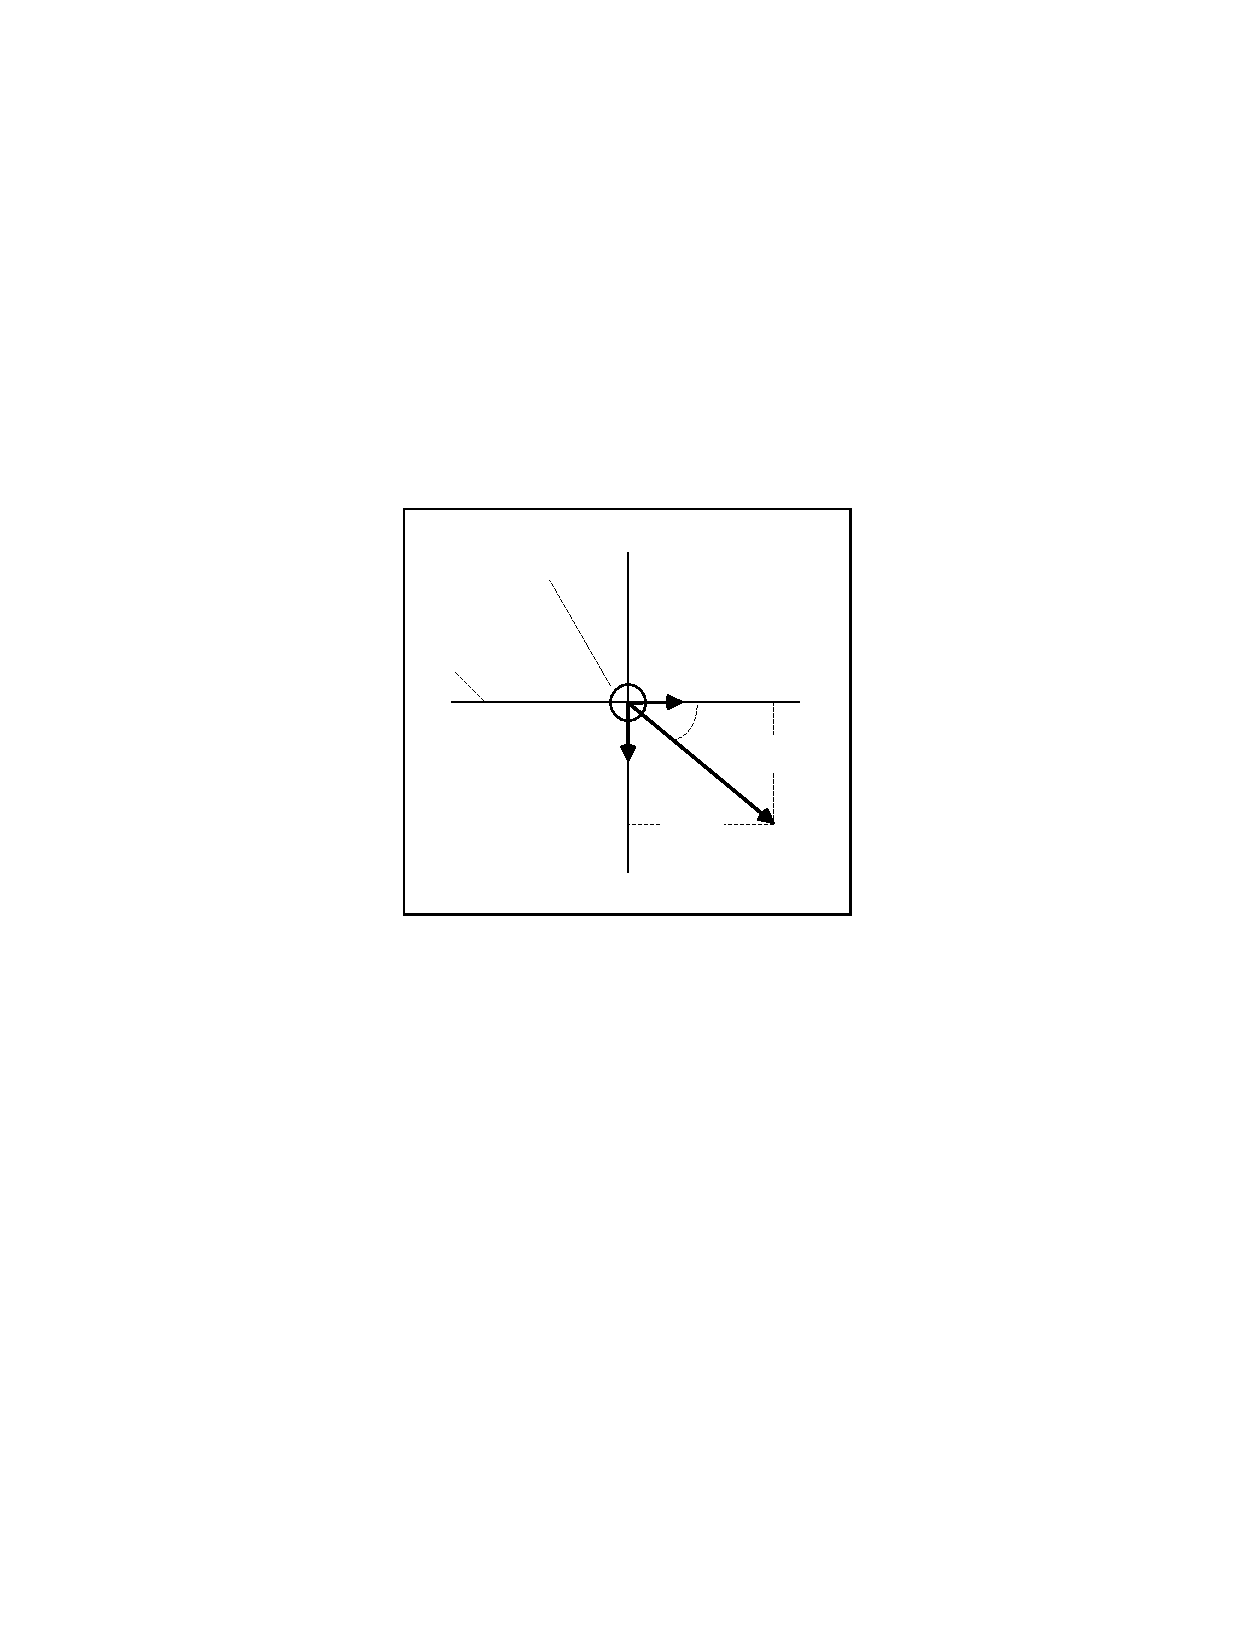
\includegraphics[scale=1]{Images/BPlaneGeometry1.eps}
    \makebox(-520,845){$\theta_B$}
    \makebox(-615,820){$\mathbf{R}$}
    \makebox(-500,810){$\mathbf{B}$}
    \makebox(-560,890){$\mathbf{T}$}
    \makebox(-760,920){$xy$-plane of $\mathcal{F}_B$ }
    \makebox(-720,990){Central Body}
    \makebox(-570,1030){$z$-axis of $\mathcal{F}_B$}
    \makebox(-580,760){$\mathbf{B}\cdot\mathbf{T}$}
    \makebox(-485,830){$\mathbf{B}\cdot\mathbf{R}$}
    \end{picture}
    \caption{Geometry of the B-Plane as Seen From a Viewpoint Perpendicular to the B-Plane}
    \label{fig:BPlaneGeometry1}
\end{figure}
%
\begin{figure}[htb]
    \begin{picture}(100,240)(265,340)
        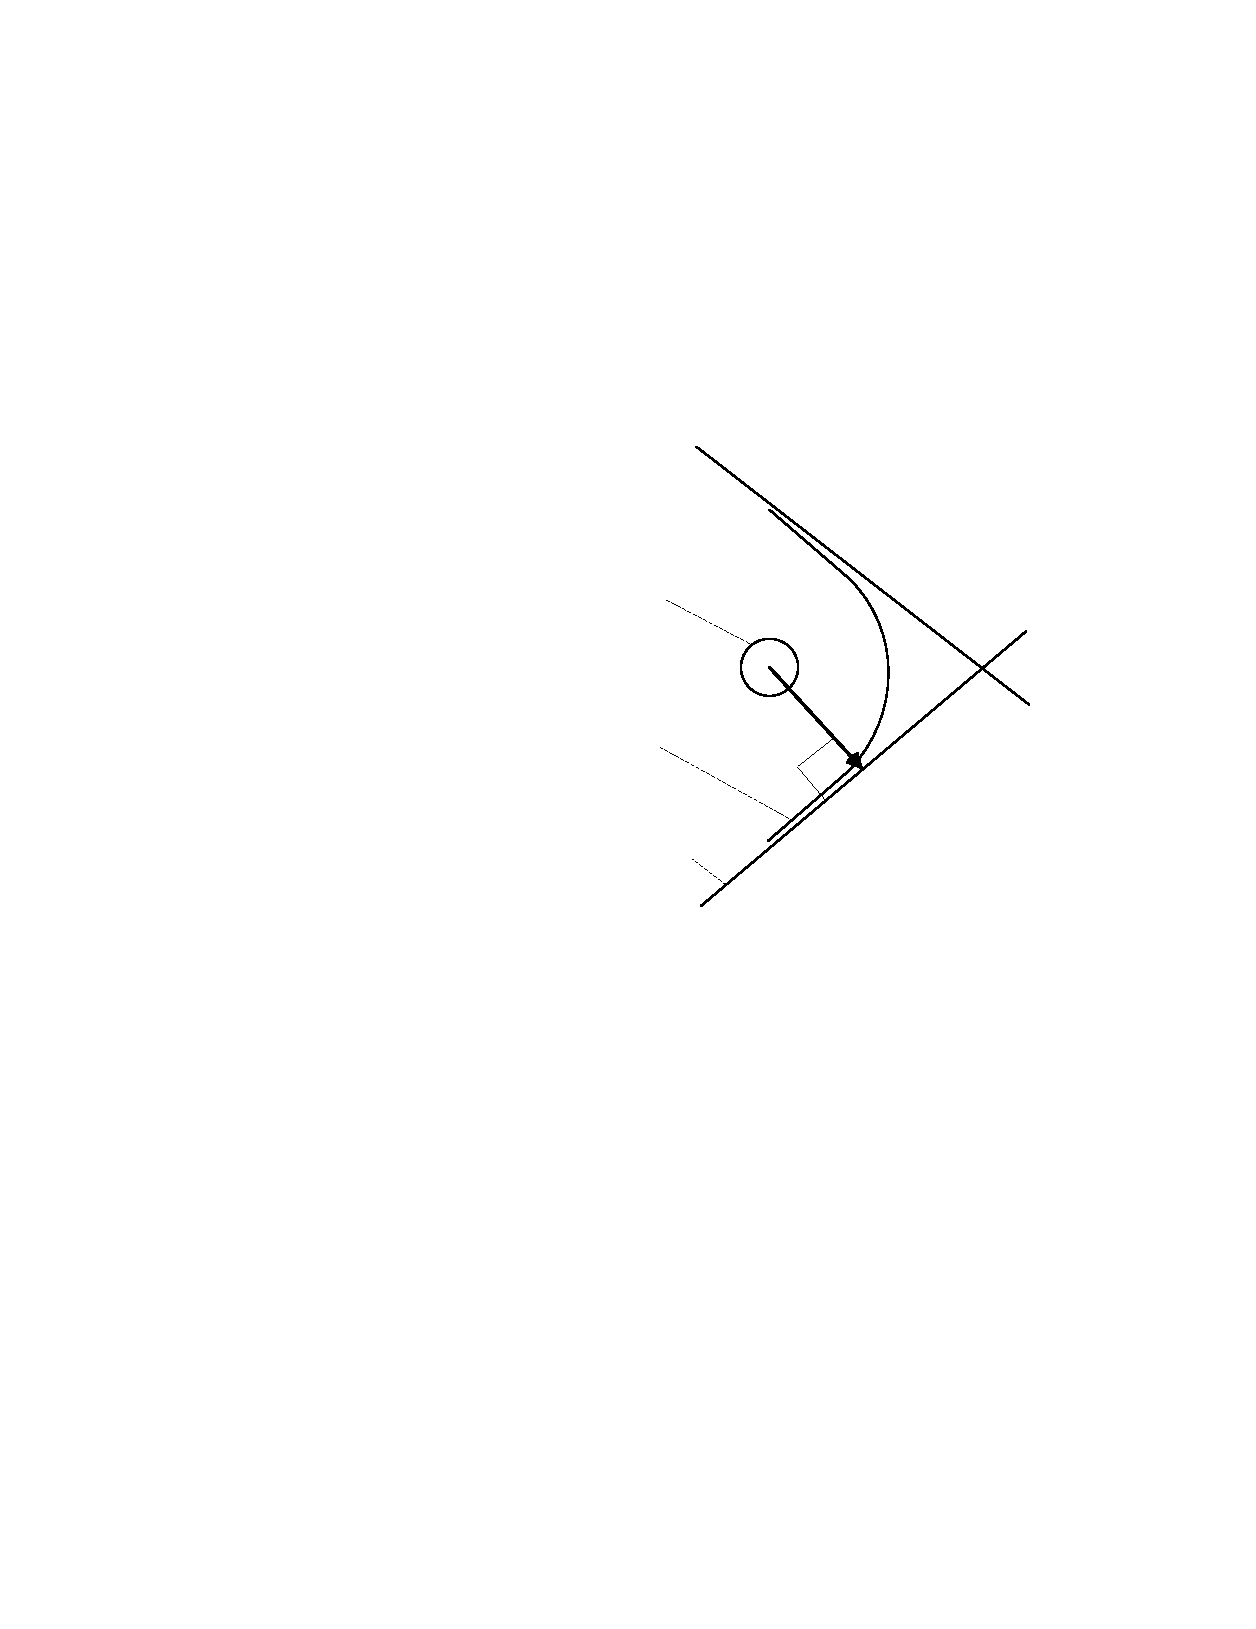
\includegraphics[scale=1]{Images/BPlaneGeometry2.eps}
    \makebox(-420,850){$\mathbf{B}$}
    \makebox(-580,990){Central Body}
    \makebox(-570,850){Incoming Trajectory}
    \makebox(-570,760){Incoming}
    \makebox(-570,740){Asymptote}
    \end{picture}
    \caption{The B-Vector as Seen From a Viewpoint Perpendicular to Orbit Plane}
    \label{fig:BPlaneGeometry2}
\end{figure}

\noindent if $\mathcal{F}_1 \neq \mathcal{F}_B$ convert $\mathbf{r}$
and $\mathbf{v}$ from $\mathcal{F}_1$ to $\mathcal{F}_B$

\[
r = \| \mathbf{r} \|
\]
%
\[
v = \| \mathbf{v} \|
\]
%
Calculate eccentricity related information
%
\[
    \mathbf{e} = \displaystyle\frac{\left( v^2 - \displaystyle\frac{\mu}{r}  \right)\mathbf{r} - (\mathbf{r} \cdot \mathbf{v})\mathbf{v}}{\mu}
\]
%
\[
   e = \| \mathbf{e} \|
\]
%
\[
\hat{\mathbf{e}} = \frac{\mathbf{e}}{e}
\]
%
If $e\leq 1$, then the method fails and returns.

Now let's calculate the angular momentum and orbit normal vectors.
%
\[
\mathbf{h} = \mathbf{r}\times \mathbf{v}
\]
%
\[
h = \| \mathbf{r}\times \mathbf{v} \|
\]
%
\[
\hat{\mathbf{h}} = \frac{\mathbf{h}}{h}
\]

A unit vector normal to both the eccentricity vector and the orbit
normal vector is defined as:
%
\[
   \hat{\mathbf{n}} = \hat{\mathbf{h}} \times \hat{\mathbf{e}}
\]
The following relations are only true for hyperbolic orbits: The
semiminor axis, $b$, can be calculated using
%
\[
   b = \frac{h^2}{\mu \sqrt{e^2 - 1}}
\]
%
The incoming asymptote is defined using
%
\[
   \mathbf{S} =  \frac{\hat{\mathbf{e}} }{e} + \sqrt{1 - \left(\frac{1}{e}\right)^2
   }\hat{\mathbf{n}}
\]
%
The B-vector, $\mathbf{B}$, is calculated using
%
\[
   \mathbf{B} = b \left(\sqrt{1 - \left(\frac{1}{e}\right)^2 }\hat{\mathbf{e}}  - \frac{1}{e} \hat{\mathbf{n}} \right)
\]
%
The remaining vectors, $\mathbf{T}$ and $\mathbf{R}$ are found using
%
\[
   \mathbf{T} = \frac{[\hspace{.03 in} S_y \hspace{.1 in} -S_x  \hspace{.1 in} 0 \hspace{.03 in}]^T }{\sqrt{S_x^2 + S_y^2}}
\]
%
\[
   \mathbf{R} = \mathbf{S} \times \mathbf{T}
\]
%
Finally, the desired quantities are found using
%
\[
   B_T = \mathbf{B} \cdot \mathbf{T}
\]
%
\[
   B_R = \mathbf{B} \cdot \mathbf{R}
\]



\noindent if  $\mathcal{F}_1 \neq \mathcal{F}_2$ , convert
$\mathbf{r}$ and $\mathbf{v}$ to $\mathcal{F}_2$
%
\begin{equation}
    A = \mathbf{r}\cdot\mathbf{v}
\end{equation}

\subsection{BetaAngle} \index{BetaAngle}

Definition:  The Beta angle, $\beta$, is defined as the angle
between the orbit normal vector, and the vector from the celestial
body to the sun.

\[
   \hat{\mathbf{h}} = \frac{  \mathbf{r}_\oplus \times \mathbf{v}_\oplus  }{\|\mathbf{r}_\oplus \times \mathbf{v}_\oplus \|}
\]
%
\[
\hat{\mathbf{r}}_{s \oplus} = \frac{\mathbf{r}_{s \oplus}}{\|_{s
\oplus }  \|}
\]
%
\begin{equation}
  \beta = \sin^{-1}\left(\hat{\mathbf{h}}\cdot \hat{\mathbf{r}}_{s\oplus } \right)
\end{equation}

\begin{itemize}
     \item $\mathbf{r}_\oplus$:  Position vector of spacecraft
     with respect to celestial body, in the EarthMJ2000Eq system.

     \item $\mathbf{v}_\oplus$:  Velocity vector of spacecraft
     with respect to celestial body, in the EarthMJ2000Eq system.

     \item $\mathbf{r}_{s\oplus}$:  Position vector from celestial
     body, to the sun.
\end{itemize}

\subsection{BVectorAngle and BVectorMag} \index{BVectorAngle}
\index{BVectorMag}

To avoid code reduplication, the magnitude and angle of the B
vector, $\|\mathbf{B}\|$ and  $\theta_B$ respectively,  are
calculated from the outputs of the B-Plane coordinates algorithm.
The equations for $\|\mathbf{B}\|$ and $\theta_B$ are
%
\begin{equation}
    \|\mathbf{B}\| = \sqrt{ B_T^2 + B_R^2}
\end{equation}
%
%
\begin{equation}
     \theta_B = \tan^{-1}{\frac{B_R}{B_T}}
\end{equation}
%
which is implemented using $atan2( B_R , B_T )$

\subsection{C3Energy}\index{Spacecraft properties!C3Energy}
\index{C3Energy}

Given:  $a$, and $\mu$

\noindent Find:  $C_3$

\begin{equation}
    C_3 = -\frac{\mu}{a}
\end{equation}

\noindent \textit{Comment}:  $a$ is calculated from the satellite
cartesian state as shown in Section \ref{Sec:Cart2Kep}, and $\mu$ is
associated with the specified central body.

\subsection{DEC} \index{DEC}

\noindent \textit{Description}: \st{DEC} is the declination of a
spacecraft, as shown in Fig. \ref{fig:SphericalElements} using the
symbol $\delta$.

\noindent \textit{Dependency}:  Coordinate System.

\noindent Given:  $\mathbf{r}$, $\mathbf{v}$ and $\mathcal{F}$

\noindent Find:  $\delta$

Begin by converting  $\mathbf{r}$ and $\mathbf{v}$ to  $\mathcal{F}$
if necessary.  Then,
%
\begin{equation}
    r = \| \mathbf{r} \|
\end{equation}
%
\begin{equation}
    \delta = \sin^{-1}(\frac{z}{r})
\end{equation}

\subsection{DECV} \index{DECV}

\noindent \textit{Description}: \st{DECV} is the declination of
velocity of a spacecraft.

\noindent \textit{Dependency}:  Coordinate System.

\noindent Given:  $\mathbf{r}$, $\mathbf{v}$ and $\mathcal{F}$

\noindent Find:  $\delta_v$

Begin by converting  $\mathbf{r}$ and $\mathbf{v}$ to  $\mathcal{F}$
if necessary.  Then,
%
\begin{equation}
       \delta_v = \sin^{-1}(\frac{v_z}{v})
\end{equation}

\subsection{ECC} \index{ECC}

\noindent \textit{Description}: \st{ECC} is the eccentricity  of an
orbit and must be greater than or equal to zero. The eccentricity
contains information on the shape of an orbit. If ECC is zero then
the orbit is circular.  If ECC is greater than zero, but less than
one, the orbit is elliptic. If ECC equals one, the orbit is
parabolic. Finally, if ECC is greater than one, the orbit is
hyperbolic.  The algorithm used in GMAT to calculate SMA is adopted
from Vallado\cite{vallado2}.

\noindent \textit{Dependency}:  Central Body.

\noindent Given:  $\mathbf{r}$, $\mathbf{v}$, and $\mu$ (Central
Body)

\noindent Find:  $e$

%
\begin{equation}
    r = \| \mathbf{r} \|
\end{equation}
%
\begin{equation}
    v = \| \mathbf{v} \|
\end{equation}
%
\begin{equation}
     \mathbf{e} = \displaystyle\frac{(v^2 - \displaystyle\frac{\mu}{r} )\mathbf{r}
     - (\mathbf{r}\cdot\mathbf{v}  )\mathbf{v}}{\mu}
\end{equation}
%
\begin{equation}
     e = \| \mathbf{e} \|
\end{equation}

\subsection{FPA} \index{FPA}

\noindent \textit{Description}: \st{FPA} is the orbit vertical
Flight Path Angle as as shown in Fig. \ref{fig:SphericalElements}
using the symbol $\psi$.

\noindent \textit{Dependency}:  Coordinate System.

\noindent Given:  $\mathbf{r}$, $\mathbf{v}$, and coordinate system
$\mathcal{F}$.

\noindent Find:  $\psi$

Begin by converting  $\mathbf{r}$ and $\mathbf{v}$ to  $\mathcal{F}$
if necessary.  Then,
%
\begin{equation}
    \psi = \cos^{-1}\left(  \frac{\mathbf{r} \cdot \mathbf{v} }{r v} \right)
\end{equation}
%

\subsection{EA} \label{sec:EccentricAnomaly}
\index{EA}

Given: $\nu$, $e$

\noindent Find:  $E$\\
%

\noindent If e $>$ ( 1 - $1e^{-11}$ ) then $E = 0$, return.\\
%


\noindent Otherwise,
%
\begin{eqnarray}
    \sin(E) & = & \frac{\sqrt{1 - e^2} \sin(\nu)}{1+e \cos{\nu}}    \\    %Vallado pg. 213,  Eq. 4-9
    %
    \cos(E) & = & \frac{ e + \cos{\nu} }{1+e \cos{\nu}}   \\     %Vallado pg. 213,  Eq. 4-9
    %
    E & = & \mbox{atan2}(\sin{E},\cos{E})
\end{eqnarray}
%

\subsection{Energy}\index{Spacecraft properties!Energy}
\index{Energy}

\noindent \textit{Description}: \st{Energy} is the orbit energy.

\noindent \textit{Dependency}:  Central Body.

\noindent Given:  $\mathbf{r}$, $\mathbf{v}$, and central body.

\noindent Find:  $\xi$

Begin by converting $\mathbf{r}$ and $\mathbf{v}$ to a coordinate
system with the origin equal to the central body defined by the
user, and the MJ2000Eq axis system.  Then,
%
\begin{equation}
     r = \mathbf{r}
\end{equation}
%
\begin{equation}
     v = \mathbf{v}
\end{equation}
%
\begin{equation}
    \xi = \frac{v^2}{2} - \frac{\mu}{r}
\end{equation}


\subsection{HMAG} \index{HMAG}

\noindent \textit{Description}: \st{HMAG} is the magnitude of the
orbit angular momentum.

\noindent \textit{Dependency}:  Central Body.

\noindent Given:  $\mathbf{r}$, $\mathbf{v}$, and central body.

\noindent Find:  $h$

Begin by converting $\mathbf{r}$ and $\mathbf{v}$ to a coordinate
system with the origin equal to the central body defined by the
user, and the MJ2000Eq axis system.  Then,
%
\begin{equation}
    \mathbf{h} = \mathbf{r} \times \mathbf{v}
\end{equation}
%
\begin{equation}
    h = \| \mathbf{h} \|
\end{equation}

\subsection{HX,HY, and HZ} \index{HX} \index{HY} \index{HZ}

\noindent \textit{Description}: \st{HX,HY,} and \st{HZ} are the
components of the orbit angular momentum vector.

\noindent \textit{Dependency}:  Coordinate System.

\noindent Given:  $\mathbf{r}$, $\mathbf{v}$, and coordinate system
$\mathcal{F}$.

\noindent Find:  $h_x$, $h_y$, and $h_z$

Begin by converting $\mathbf{r}$ and $\mathbf{v}$ to $\mathcal{F}$
if necessary. Then,
%
\begin{equation}
    \mathbf{h} = \mathbf{r} \times \mathbf{v} = [\hspace{.05 in} h_x
    \hspace{.1 in} h_y \hspace{.1 in} h_z \hspace{.05 in} ]^T
\end{equation}


\subsection{HA}  \label{sec:HyperbolicAnomaly}
\index{HA}

\noindent \textit{Description}: \st{HA} is the orbit Hyperbolic
Anomaly and is only defined for hyperbolic orbits.  For
non-hyperbolic orbits, \st{HA} returns a value of zero.

\noindent \textit{Dependency}:  Central Body.
 Given: $\nu$, $e$

\noindent Find:  $H$\\
%

\noindent If e $<$ ( 1 + $1e^{-11}$ ) then $H = 0$, return.\\
%


\noindent Otherwise,
%
\begin{eqnarray}
    \sinh(H) & = & \frac{ \sin(\nu) \sqrt{e^2 - 1}}{1+e \cos{\nu}}    \\    %Vallado pg. 213,  Eq. 4-9
    %
    \cosh(H) & = & \frac{ e + \cos{\nu} }{1+e \cos{\nu}}   \\     %Vallado pg. 213,  Eq. 4-9
    %
    H & = & \tanh^{-1}(\frac{\sinh{H}}{\cosh{H}})
\end{eqnarray}
%

\subsection{INC} \index{INC}

\noindent \textit{Description}: \st{INC} is the inclination of an
orbit in the chosen coordinate system.

\noindent \textit{Dependency}:  Coordinate System.

\noindent Given:  $\mathbf{r}$, $\mathbf{v}$, and coordinate system
$mathcal{F}$.

\noindent Find:  $e$

Begin by converting  $\mathbf{r}$ and $\mathbf{v}$ to  $mathcal{F}$
if necessary.  Then,
%
\begin{equation}
     \mathbf{h} = \mathbf{r} \times \mathbf{v}
\end{equation}
%
\begin{equation}
      h  = \mathbf{h}
\end{equation}
%
\begin{equation}
     i = \cos^{-1}( \frac{h_z}{h} )
\end{equation}


\subsection{Latitude} \label{Sec:Latitude} \index{Latitude}

\noindent \textit{Description}: \st{Latitude} is the geodetic
latitude of a spacecraft.  The geodedic latitude is defined as the
the angle $\phi_{gc}$, as shown in Fig. ( ),  where the
sub-satellite point is defined by the interscection of a line drawn
from the spacecraft and perpendicular to a plane tangent to the
surface of the body. GMAT assumes the body is an ellipsoid. The
equatorial radius, and properties of the ellipsoid depend upon the
particular body chosen by the user.  The algorithm in GMAT is taken
from Vallado\cite{vallado2}.

\begin{figure}[htb]
    \begin{picture}(100,200)(185,310)
        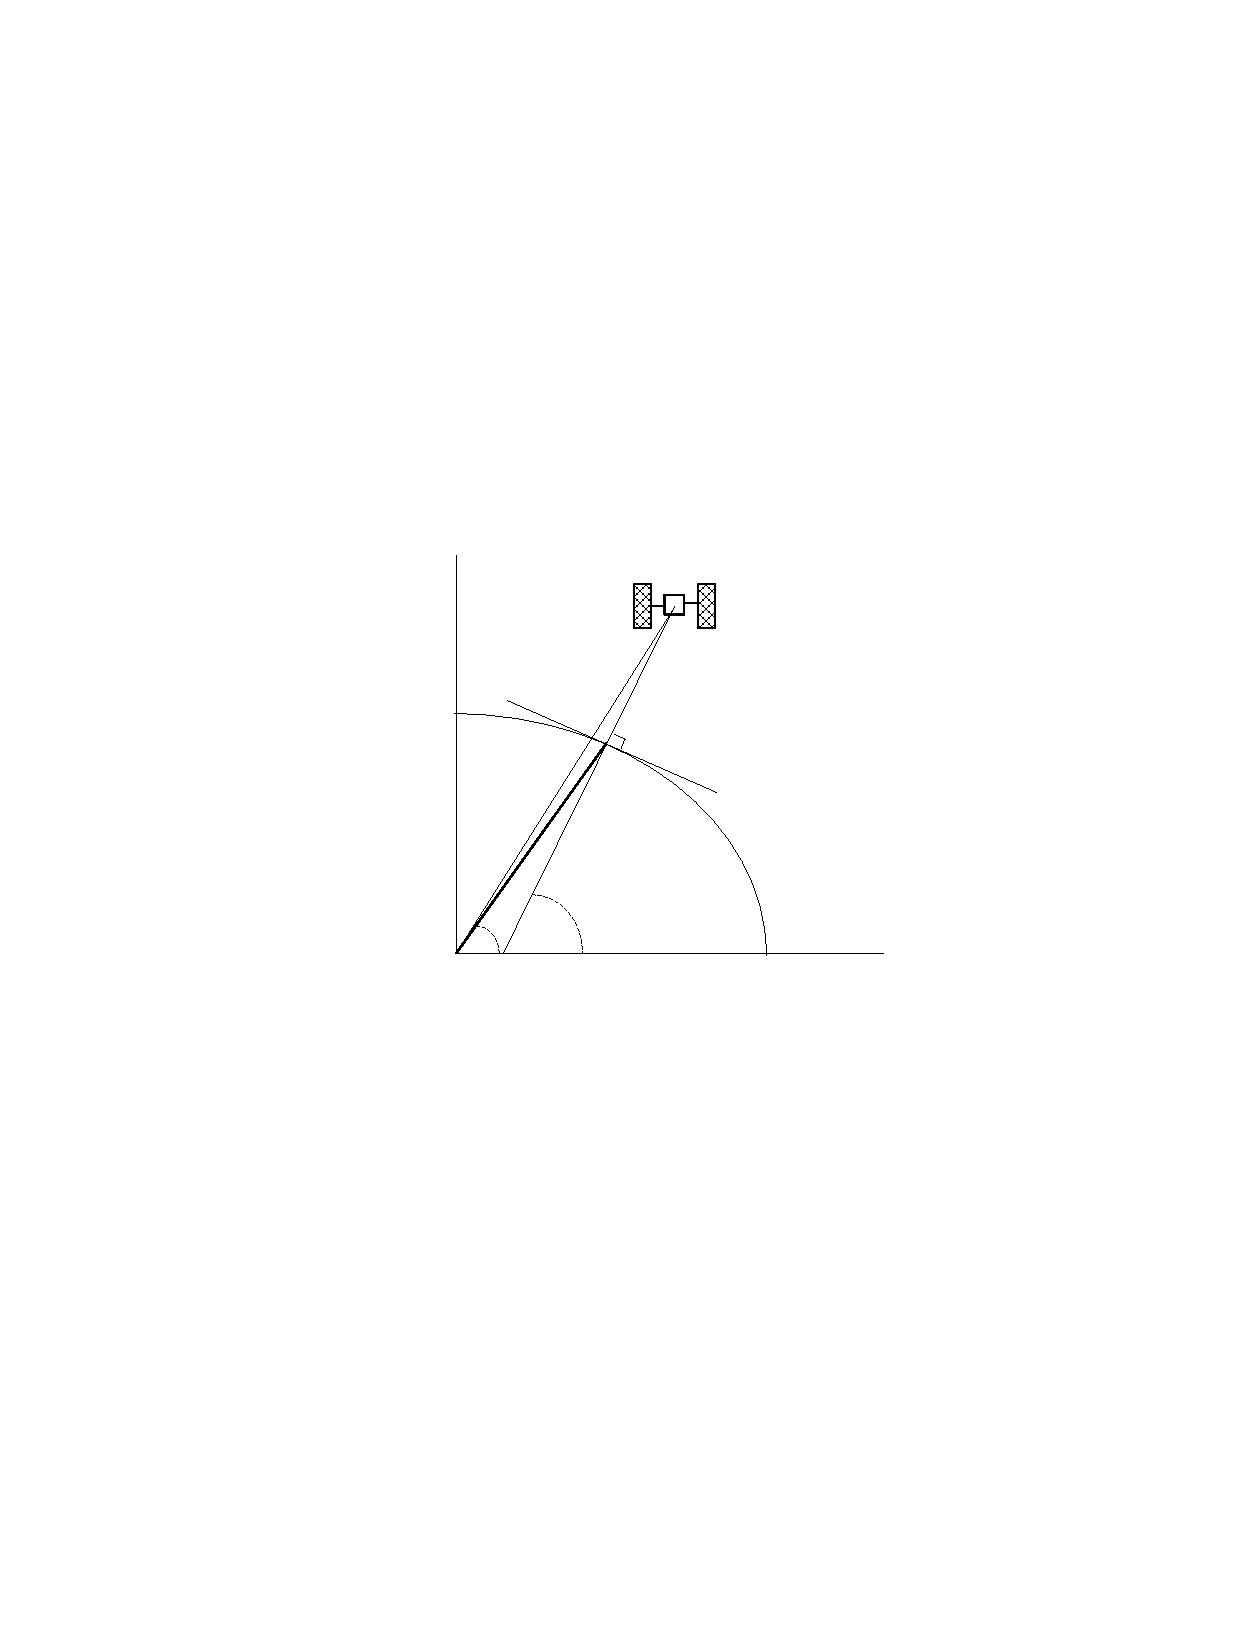
\includegraphics[scale=1]{Images/GeodeticDiagram.eps}
    \makebox(-575,880){$h$}
    \makebox(-640,680){$\phi_{gd}$}
    \makebox(-730,670){$\phi_{gc}$}
    \end{picture}
    \caption{Geocentric and Geodetic Latitude}
    \label{fig:GeodeticDiagram}
\end{figure}

\noindent \textit{Dependency}:  Central Body.

\noindent Given:  $\mathbf{r}$ in $\mathcal{F}_1$

\noindent Find:  $\phi_{gc}$

\noindent Definitions:
\begin{itemize}
     %
     \item $\mathcal{F}_1$ is the coordinate system in which GMAT originally knows $\mathbf{r}$
     %
     \item $\mathcal{F}_F$ is body fixed system of the central body selected by the user.
     %
     \item $f$ is the bodies flattening coefficient
     %
     \item $R$ is the bodies mean equatorial radius
     %
     \item $\phi_{gd}$ is the geodedic latitude of the spacecraft
     in the body fixed frame.
     %
\end{itemize}
%
if $\mathcal{F}_1 \neq \mathcal{F}_F$ convert $\mathbf{r}$ from
$\mathcal{F}_1$ to $\mathcal{F}_F$. Then,
%
\begin{equation}
     r_{xy} = \sqrt{ x^2 + y^2 }
\end{equation}
%
Calculate the geocentric latitude to use as an initial guess to find
the geodetic latitude
%
\begin{equation}
     \phi_{gd}  \approx \mbox{atan2}(z,  r_{xy}  );
\end{equation}
%
\begin{equation}
    e^2 = 2f-f^2
\end{equation}
%

\noindent Set $\delta = 1.0$ to initialize the loop, then,


\noindent While ( $\delta > 10^{-7}$ )
%
\begin{eqnarray}
   \phi' & = & \phi_{gd}\\
   %c & = & \frac{R} { \sqrt{1 - e^2\sin{\phi}}    }\\
   \phi_{gd} & = & \mbox{atan2}\left(z +  \frac{Re^2\sin^{2}{\phi_{gd}}} { \sqrt{1 - e^2\sin{\phi_{gd}}} }, r_{xy}
   \right)\\
   \delta & = & | \phi_{gd} - \phi' |
\end{eqnarray}
%
EndWhile\\
%

After convergence, $\phi_{gd}$ is converted to degrees, and
converted to fall between $-90^\circ$ and   $+90^\circ$ degrees.

\subsection{Longitude} \label{Sec:CalcObjectLongitude}
\index{Longitude}

\noindent \textit{Description}: \st{Longitude} is the longitude of
an object, in the body fixed frame of the central body chosen by the
user.

\noindent \textit{Dependency}:  Central Body.

\noindent Given:  $\mathbf{r}$, central body.

\noindent Find:  $\phi$

Begin by converting $\mathbf{r}$ to the body fixed system of the
central body defined by the user. Then,
%
\begin{equation}
    \phi = \tan_2^{-1}(y,x);
\end{equation}
%
The calculation is completed by converting to degrees and setting
the value to such that $-180 \leq \phi < 180$.

\subsection{LST} \index{LST}

\noindent \textit{Description}: \st{LST} is the local sidereal time
of an object, with respect to the selected central body.  The local
sidereal time is the sum of the longitude in the bodies fixed frame,
and the mean sidereal time.  This is illustrated in Fig.
\ref{fig:SiderealTimeDiagram}, where $\mathcal{F}_I$ is the body's
equatorial inertial system (as described in Sec. \ref{Sec:Equator}),
$\mathcal{F}_F$ is the body's fixed system (as described in Sec.
\ref{Sec:Fixed}).  $\lambda$ is the longitude of the object, in this
case a spacecraft, and $\theta_{MST}$ is the mean sidereal time of
the prime meridian.

\noindent \textit{Dependency}:  Central Body.

\noindent Given:  $\mathbf{r}$, $t_i$ (epoch of spacecraft in
internal time system), and central body

\noindent Find:  $\theta_{LST}$

\noindent Definitions:
\begin{itemize}
     %
     \item $\mathcal{F}_I$ equatorial inertial system (as described in Sec. \ref{Sec:Equator}) of selected central
     body.
     %
     \item $\mathcal{F}_F$ is the central body's fixed system (as described in Sec. \ref{Sec:Fixed})
     %
     \item $\lambda$ is the longitude of the object in $\mathcal{F}_F$
     %
     \item $\theta_{MST}$ is the mean sidereal time of the central body's  prime meridian.
     %
     \item $t_i$ (epoch of spacecraft in internal time system)
\end{itemize}

\begin{figure}[htb]
    \begin{picture}(100,230)(185,460)
        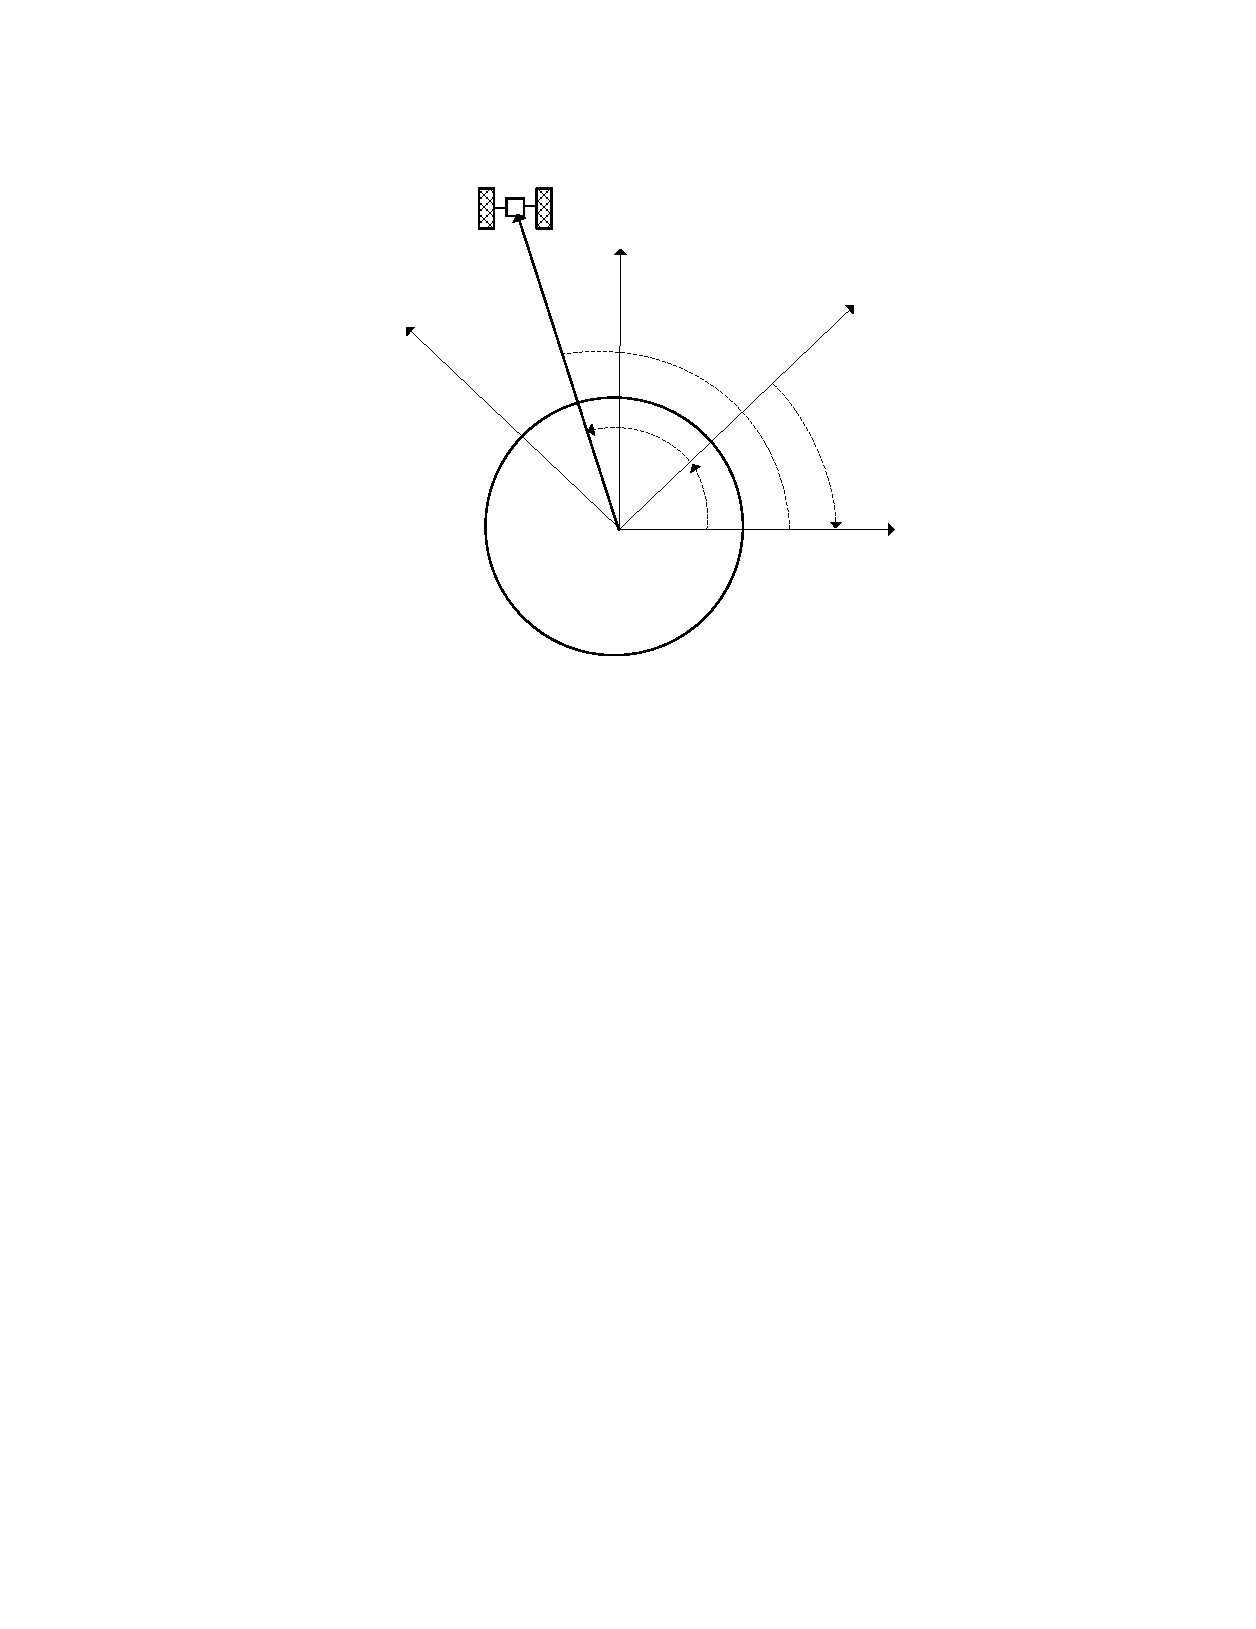
\includegraphics[scale=1]{Images/SiderealTimeDiagram.eps}
    \makebox(-350,1066){$\hat{\mathbf{x}}_I$}
    \makebox(-380,1277){$\hat{\mathbf{x}}_F$}
    \makebox(-617,1330){$\hat{\mathbf{y}}_I$}
    \makebox(-800,1240){$\hat{\mathbf{y}}_F$}
    \makebox(-575,1059){$\theta_{MST}$}
    \makebox(-600,1120){$\lambda$}
    \makebox(-580,1220){$\theta_{LST}$}
    \makebox(-425,1125){$\theta_{MHA}$}
    \end{picture}
    \caption{Local Sidereal Time Geometry}
    \label{fig:SiderealTimeDiagram}
\end{figure}

We begin by calculating $\lambda$ using the algorithm described in
Sec. \ref{Sec:CalcObjectLongitude}.  The mean sidereal time
$\theta_{MST}$ is calculated differently for Earth than for other
central bodies.  If the central body is Earth, then we use the
following equations to calculate $\theta_{MST}$.

First, convert $t_i$, which is the spacecraft epoch in the interal
time system (A1 Modified Julian Date), to $T_{UT1}$, which is the
number elapsed Julian centuries from the J2000 epoch.
%
\begin{equation}
    T_{UT1} = \frac{t_{ut1} - 21544.5}{36525}
\end{equation}
%
\begin{equation}\begin{split}
    \theta_{MST} =  & 67310.54841^s + \\ &( 876600^h \left( \frac{3600 s}{1h}\right) + 8640184.812866)T_{UT1} + \\& 0.093104T_{UT1}^2 - 6.2\times10^{-6}T_{UT1}^3
    \end{split}
\end{equation}

\subsection{MA} \index{MA}

Given: $\nu$, $e$

\noindent Find:  $M$

\noindent If e $<$ ( 1 - $1e^{-11}$ ) then calculate $E$ using
algorithm in Sec. \ref{sec:EccentricAnomaly}.  Then $M$ is
calculated using
%
\begin{equation}
     M = E - e \sin{E}
\end{equation}
%
Note: $E$ must be expressed in radians in the above equation, and
results in $M$ in radians.

\noindent If e $>$ ( 1 + $1e^{-11}$ ) then calculate $H$ using
algorithm in Sec. \ref{sec:HyperbolicAnomaly}.  Then $M$ is
calculated using
%
\begin{equation}
     M =  e \sinh{H} - H
\end{equation}
%
Note: $H$ must be expressed in radians in the above equation, and
results in $M$ in radians.  GMAT outputs \st{MA} in degrees.

\noindent If neither of the above conditions are satisfied, $M = 0$,
and output ``Warning:  Orbit is near parabolic in mean anomaly
calculation. Setting MA = 0".

\subsection{MHA}

\subsection{MM}\index{Spacecraft properties!mean motion}
\index{MM}

Given:  $a$, $e$, and $\mu$

\noindent Find:  $n$

\noindent The orbit is considered either circular or elliptic ( both
orbit types use the same equation to calculate $n$) if $ e < 1 -
1e^{-11}$. In this case the mean motion, $n$, is calculated using
%
\begin{equation}
    n = \sqrt{\frac{\mu}{a^3}}
\end{equation}
%
The orbit is considered hyperbolic if $ e > 1 + 1e^{-11}$.  In this
case the mean motion, $n$, is calculated using
%
\begin{equation}
    n =  \sqrt{-\frac{\mu}{a^3}}
\end{equation}
%
If neither of the above two conditions are met, the mean motion is
calculated using
%
%
\begin{equation}
    n =  2\sqrt{\mu}
\end{equation}
%

\noindent \textit{Comment}:  $a$ and $e$ are calculated from the
satellite cartesian state as shown in Section \ref{Sec:Cart2Kep},
and $\mu$ is associated with the specified central body.


\subsection{OrbitPeriod}\index{Spacecraft properties!OrbitPeriod}
\index{OrbitPeriod}

Given:  $a$, and $\mu$

\noindent Find:  $T$

\noindent If a $ < 0$,  then $T = 0$, return.\\
%


\noindent Otherwise,
\begin{equation}
    T = 2\pi\sqrt{\frac{a^3}{\mu}}
\end{equation}

\noindent \textit{Comment}:  $a$ is calculated from the satellite
cartesian state as shown in Section \ref{Sec:Cart2Kep}, and $\mu$ is
associated with the specified central body.

\subsection{PercentShadow } \label{sec:PercentShadow}
\index{PercentShadow}

The \st{PercentShadow} parameter calculates the percentage of the
apparent solar disk that is in view from the perspective of a
spacecraft. The algorithm used in GMAT was adapted from
Montenbruck\cite{Montenbruck:Gill:05} pgs. 80-83.

\begin{figure}[htb]
    \begin{picture}(100,220)(175,275)
        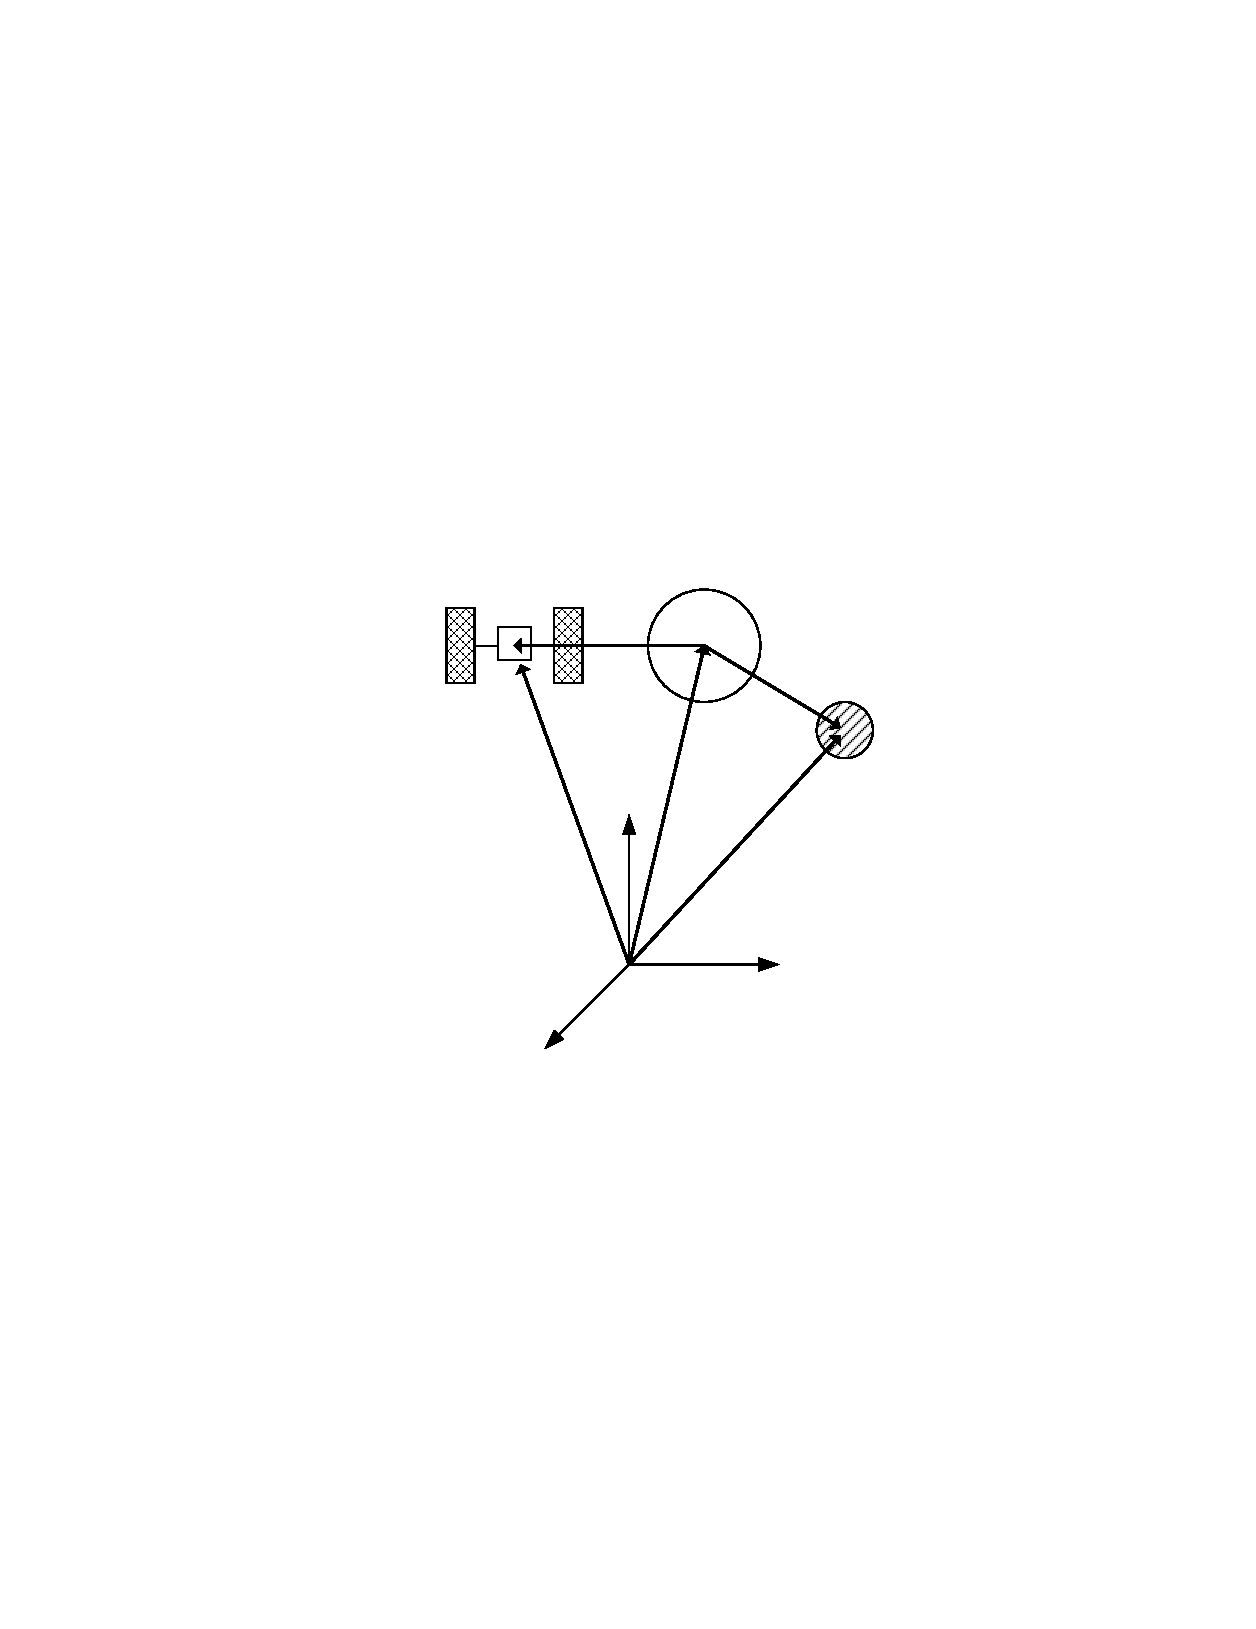
\includegraphics[scale=1]{Images/ShadowGeometry.eps}
    \makebox(-520,850){$\mathbf{r}_B$}
    \makebox(-460,750){$\mathbf{r}_\odot$}
    \makebox(-690,800){$\mathbf{r}$}
     \makebox(-620,940){$\mathbf{s}$}
     \makebox(-450,890){$\mathbf{s}_\odot$}
    \end{picture}
    \caption{Shadow Geometry}
    \label{fig:ShadowGeometry}
\end{figure}
%
\begin{itemize}
    \item $R_\odot$ = Radius of the Sun
    \item $R_B$ = Radius of occulting body
    \item $R'_\odot$ = Apparent radius of the Sun
    \item $R'_B$ = Apparent radius of occulting body
    \item $\mathbf{r}_\odot$ = Vector from central body to Sun
    \item $\mathbf{r}_B$ = Vector from central body to occulting body
    \item $\mathbf{r}$ = Vector from central body to s/c
\end{itemize}
%

We begin by calculating the vector from the occulting body to the
spacecraft, $\mathbf{s}$, using
%
\begin{equation}
     \mathbf{s} = \mathbf{r} - \mathbf{r}_B
\end{equation}
%
and the vector from the occulting body to the sun,
$\mathbf{s}_\odot$, using
%
\begin{equation}
     \mathbf{s}_\odot = \mathbf{r}_\odot - \mathbf{r}_B
\end{equation}
%
(Note that when the occulting body is the same as the central body,
$\mathbf{s} = \mathbf{r}$, and $\mathbf{s}_\odot =
\mathbf{r}_\odot$)

Next we calculate the apparent radius of the Sun and occulting body
using
%
\begin{eqnarray}
     R'_\odot & = & \sin^{-1}\frac{R_\odot}{\|\mathbf{r}_\odot - \mathbf{r} \|}\\
     R'_B & = & \sin^{-1}\frac{R_B}{\|\mathbf{r}  - \mathbf{r}_B\|}
\end{eqnarray}
%
We can calculate the apparent separation of the two bodies, $D'$,
using
%
\begin{equation}
    D' = \cos^{-1}\left(\frac{-\mathbf{s}^T\left( \mathbf{r}_\odot - \mathbf{r} \right)}{s \|\mathbf{r}_\odot - \mathbf{r}
    \|}\right)
\end{equation}
%

If $ D' \geq R'_\odot + R'_B $, then the spacecraft is not in the
body's shadow and
%
\begin{equation}
    p = 0;
\end{equation}
%

If $D' \leq R'_B - R'_\odot$, then the spacecraft is in full shadow
and
%
\begin{equation}
    p = 100;
\end{equation}
%

If neither of the above conditions are met, the spacecraft is in
partial shadow.
%
\begin{figure}[htb]
    \begin{picture}(100,135)(135,355)
        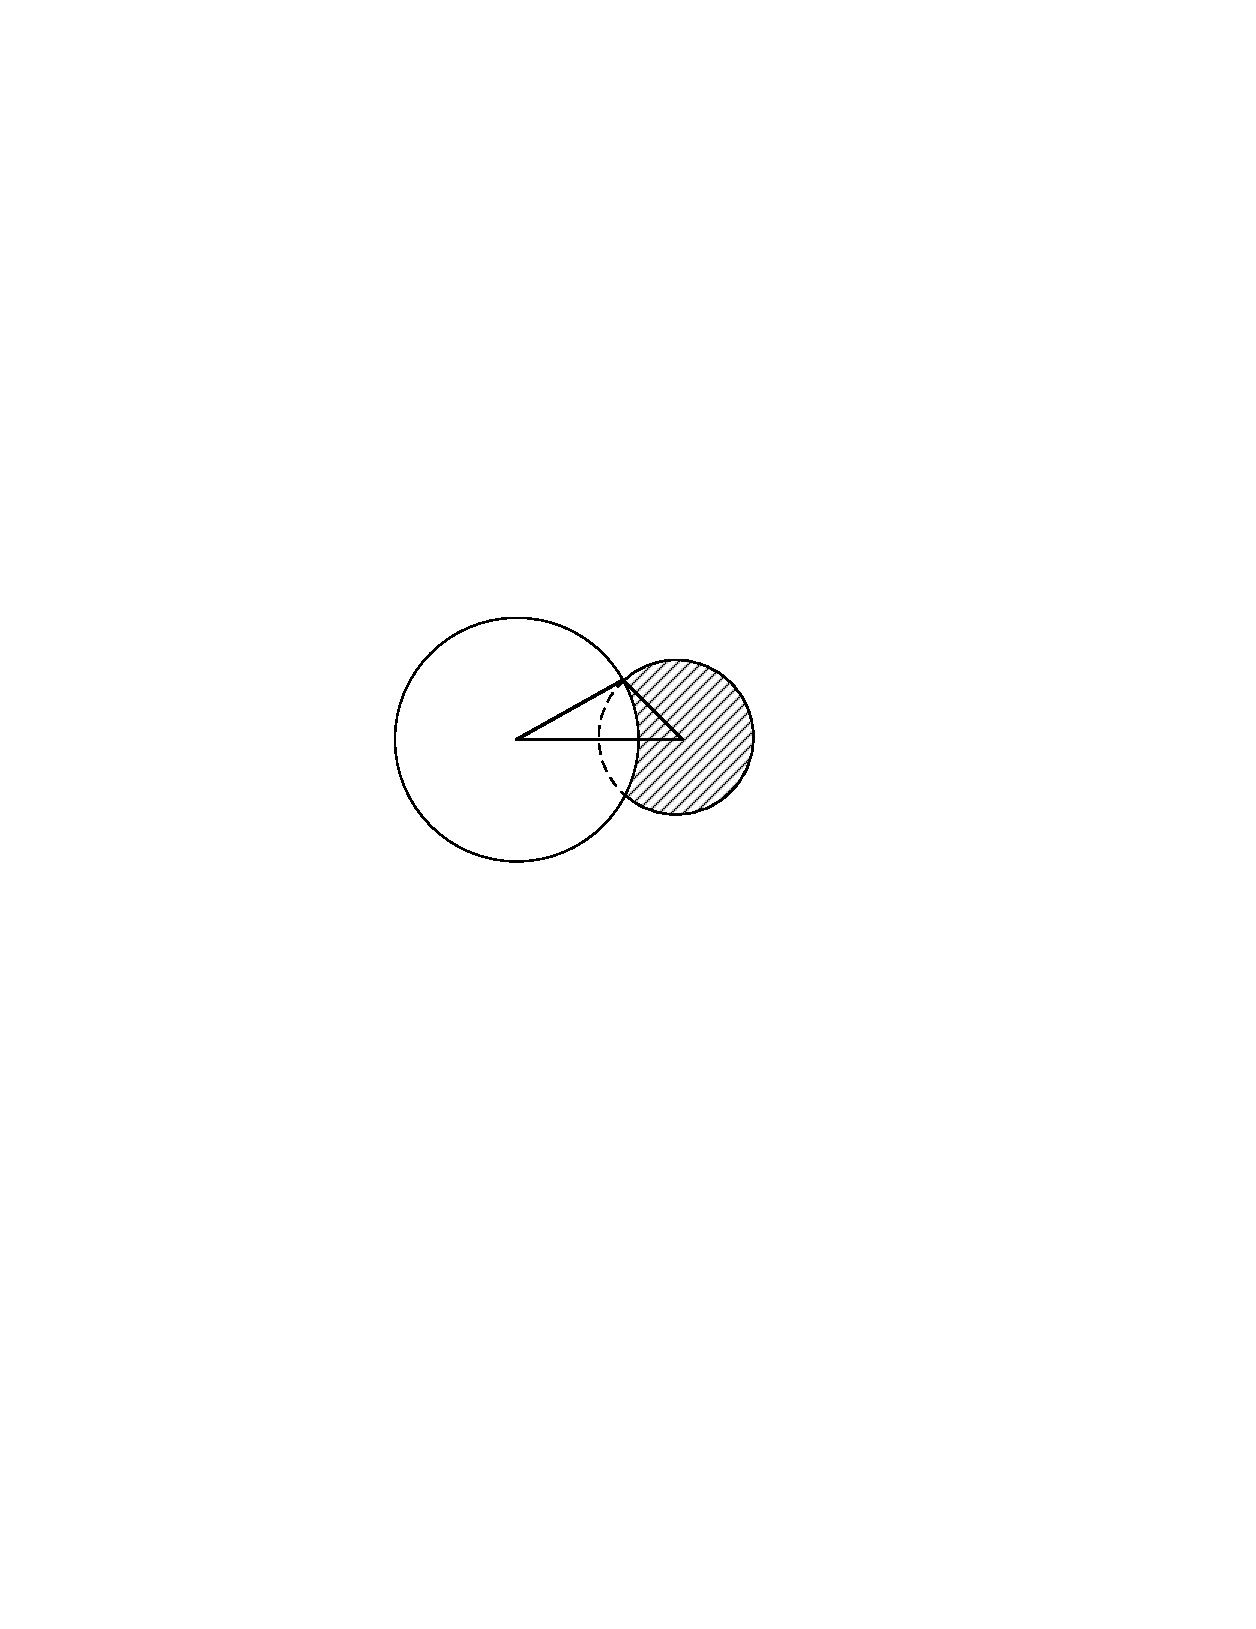
\includegraphics[scale=1]{Images/ShadowIllustration.ps}
            \makebox(-650,895){$R'_B$}
            \makebox(-550,870){$R'_\odot$}
            \makebox(-670,820){$D'$}
            \makebox(-560,750){Sun}
            \makebox(-720,765){Occulting Body}
    \end{picture}
    \caption{Occultation Geometry in Calculation of PercentShadow}
    \label{fig:ShadowIllustration}
\end{figure}
%

If $|R'_s - R'_B| < D' < R'_s + R'_B$, then we can calculate the
percentage of shadow by calculating the area of overlap, $A$,  of
the two apparent disks as shown in Fig.
\ref{fig:ShadowIllustration}.
%
\begin{equation}
     A = R^{'\mbox{} 2}_\odot\cos^{-1}\left(\frac{c_1}{R'_\odot}\right) +
     R^{'\mbox{} 2}_B\cos^{-1}\left(\frac{D' - c_1}{R'_B}\right) -
     D'c_2
\end{equation}
%
where
%
\begin{equation}
   c_1 = \frac{ D^{'\mbox{} 2} + R^{'\mbox{} 2}_\odot - R^{'\mbox{} 2}_B }{2D'}
\end{equation}
%
and
%
\begin{equation}
   c_2 = \sqrt{ R^{'\mbox{} 2}_\odot -  c_1^2 }
\end{equation}
%
The percent  shadow can be calculated using
%
\begin{equation}
     p = 100 \frac{A}{\pi R^{'\mbox{} 2}_\odot}
\end{equation}

If the condition $|R'_\odot - R'_B| < D' < R'_\odot + R'_B$ is not
satisfied, then the eclipse is annular and we use
%
\begin{equation}
     p = 100   \frac{R^{'\mbox{} 2}_B}{R^{'\mbox{} 2}_\odot}
\end{equation}


\subsection{RA}\index{RA}

\noindent \textit{Description}: \st{RA} is the right ascension of a
spacecraft, as shown in Fig. \ref{fig:SphericalElements} using the
symbol $\lambda$.

\noindent \textit{Dependency}:  Coordinate System.

\noindent Given:  $\mathbf{r}$, $\mathbf{v}$ and $\mathcal{F}$

\noindent Find:  $\lambda$

Begin by converting  $\mathbf{r}$ and $\mathbf{v}$ to  $\mathcal{F}$
if necessary.  Then,
%
\begin{equation}
    \lambda= \tan^{-1}_2(y,x)
\end{equation}

\subsection{RAV} \index{RAV}

\noindent \textit{Description}: \st{RAV} is the right ascension of
velocity of a spacecraft, as shown in Fig.
\ref{fig:SphericalElements} using the symbol $\lambda_v$.

\noindent \textit{Dependency}:  Coordinate System.

\noindent Given:  $\mathbf{r}$, $\mathbf{v}$ and $\mathcal{F}$

\noindent Find:  $\lambda_v$

Begin by converting  $\mathbf{r}$ and $\mathbf{v}$ to  $\mathcal{F}$
if necessary.  Then,
%
\begin{equation}
    \lambda_v= \tan^{-1}_2(v_y,v_x)
\end{equation}


\subsection{RAAN} \index{RAAN}

\noindent \textit{Description}: \st{RAAN} is the right ascension of
the ascending node as shown in Fig. \ref{fig:KeplerianElements}
using the symbol $\Omega$.

\noindent \textit{Dependency}:  Coordinate System.

\noindent Given:  $\mathbf{r}$, $\mathbf{v}$, and coordinate system
$\mathcal{F}$.

\noindent Find:  $e$

Begin by converting  $\mathbf{r}$ and $\mathbf{v}$ to  $\mathcal{F}$
if necessary.  Then,
%First calculate the specific angular momentum and its magnitude.
\begin{equation}
     \mathbf{h} = \mathbf{r} \times \mathbf{v}
\end{equation}
%
\begin{equation}
     h = \|\mathbf{h} \|
\end{equation}
%
\begin{equation}
     \mathbf{n} = [ \hspace{0.05 in} 0 \hspace{0.1 in} 0 \hspace{0.1 in} 1 \hspace{0.05
     in}]^T \times \mathbf{h}
\end{equation}
%
\begin{equation}
     n = \| n\|
\end{equation}
%
\begin{equation}
     i = \cos^{-1}\left(\frac{h_z}{h}\right)
\end{equation}
%


\noindent if  $(i \geq 10^{-11})$, then
%
\begin{equation}
    \Omega = \cos^{-1}\left(\frac{n_x}{n}\right)
\end{equation}
%
Fix quadrant for $\Omega$: if $n_y < 0$, then $\Omega = 2\pi -
\Omega$


\noindent if  $(i < 10^{-11})$, then
%
\begin{equation}
    \Omega = 0
\end{equation}


\subsection{RadApo}\index{Spacecraft properties!RadApo}
\index{RadApo}

Given:  $a$, and $e$

\noindent Find:  $r_a$

\noindent  if $ 1 - e  < 10^{-12}$  then $r_a = 0$.  Note, this
means that for parabolica, and hyperbolic orbits, GMAT outputs a
value of zero for \st{RadApo}.
%
\noindent Otherwise,
%
\begin{equation}
    r_a = a(1+e)
\end{equation}

\noindent \textit{Comment}:  $a$ and $e$ are calculated from the
satellite cartesian state as shown in Section \ref{Sec:Cart2Kep}.

\subsection{RadPer}\index{Spacecraft properties!RadPer}
\index{RadPer}

Given:  $a$, and $e$

\noindent Find:  $r_p$

\begin{equation}
    r_p = a(1-e)
\end{equation}

\noindent \textit{Comment}:  $a$ and $e$ are calculated from the
satellite cartesian state as shown in Section \ref{Sec:Cart2Kep}.

\subsection{RMAG} \index{RMAG}

\noindent \textit{Description}: \st{RMAG} is the magnitude of the
spacecraft's position vector.

\noindent \textit{Dependency}:  Central Body.

\noindent Given:  $\mathbf{r}$ and central body.

\noindent Find:  $r$

Begin by converting $\mathbf{r}$  to a coordinate system with the
origin equal to the central body defined by the user, and the
MJ2000Eq axis system.  Then,
%
\begin{equation}
    r = \| \mathbf{r} \|
\end{equation}

\subsection{SemilatusRectum} \index{SemilatusRectum}

\noindent \textit{Description}: \st{SemilatusRectum} is the orbit
semilatus rectum, which is the magnitude of the position vector,
when at true anomaly of $90^{\circ}$.

\noindent \textit{Dependency}:  Central Body.

\noindent Given:  $\mathbf{r}$, $\mathbf{v}$, and $\mu$ (central
body).

\noindent Find:  $p$

Begin by converting $\mathbf{r}$ and $\mathbf{v}$ to a coordinate
system with the origin equal to the central body defined by the
user, and the MJ2000Eq axis system.  Then,
%
\begin{equation}
    \mathbf{h} = \mathbf{r} \times \mathbf{v}
\end{equation}
%
\begin{equation}
    h = \| \mathbf{h} \|
\end{equation}
%
\begin{equation}
    p = \frac{h^2}{\mu}
\end{equation}


\subsection{SMA} \index{SMA}

\noindent \textit{Description}: \st{SMA} is the semimajor axis  of
an orbit. The SMA contains information on the size and type of an
orbit.  If the SMA is positive, the orbit is elliptic.  If the SMA
is negative the orbit is hyperbolic.  The SMA is undefined for
parabolic orbits. The algorithm used in GMAT to calculate SMA is
adopted from Vallado\cite{vallado2}.

\noindent \textit{Dependency}:  Central Body.

\noindent Given:  $\mathbf{r}$, $\mathbf{v}$, and $\mu$ (Central
Body)

\noindent Find:  $a$


%
\begin{equation}
    r = \| \mathbf{r} \|
\end{equation}
%
\begin{equation}
    v = \| \mathbf{v} \|
\end{equation}
%
\begin{equation}
     \xi = \frac{v^2}{2} - \frac{\mu}{r}
\end{equation}
%
if $|1 - e| > 10^{-30}$, then
\begin{equation}
     a = -\frac{\mu}{2\xi}
\end{equation}
%
otherwise, report  error and return.  Error: ``Warning: Orbit is
near parabolic and SMA is undefined".

\subsection{TA} \index{TA}

\noindent \textit{Description}: \st{TA} is the orbit true anomaly as
shown in Fig. \ref{fig:KeplerianElements} using the symbol $\nu$.

\noindent \textit{Dependency}:  Central Body.

\noindent Given:  $\mathbf{r}$, $\mathbf{v}$, and coordinate system
$\mathcal{F}$.

\noindent Find:  $\nu$

Begin by converting  $\mathbf{r}$ and $\mathbf{v}$ to  $\mathcal{F}$
if necessary.  Then,
%First calculate the specific angular momentum and its magnitude.
\begin{equation}
     \mathbf{h} = \mathbf{r} \times \mathbf{v}
\end{equation}
%
\begin{equation}
     h = \|\mathbf{h} \|
\end{equation}
%
\begin{equation}
     \mathbf{n} = [ \hspace{0.05 in} 0 \hspace{0.1 in} 0 \hspace{0.1 in} 1 \hspace{0.05
     in}]^T \times \mathbf{h}
\end{equation}
%
\begin{equation}
     n = \| n\|
\end{equation}
%
\begin{equation}
    r = \| \mathbf{r} \|
\end{equation}
%
\begin{equation}
    v = \| \mathbf{v} \|
\end{equation}
%
\begin{equation}
     \mathbf{e} = \displaystyle\frac{(v^2 - \displaystyle\frac{\mu}{r} )\mathbf{r} - (\mathbf{r}\cdot\mathbf{v}  )\mathbf{v}}{\mu}
\end{equation}
%
\begin{equation}
     e = \| \mathbf{e} \|
\end{equation}
%
\begin{equation}
     i = \cos^{-1}\left(\frac{h_z}{h}\right)
\end{equation}
%
There are three special cases, and they are treated differently.

\noindent\textit{Special Case 1:  Elliptic Orbit  }

\noindent if $(e \geq 10^{-11})$, then
%
\begin{equation}
    \nu = \cos^{-1}\left( \frac{\mathbf{e}\cdot\mathbf{r}}{er}\right)
\end{equation}
%
Fix quadrant for $\nu $:  if $\mathbf{r} \cdot \mathbf{v} < 0$, then
$\nu = 2\pi - \nu$

\noindent\textit{Special Case 2:  Circular, Inclined Orbit  }

\noindent if $(e < 10^{-11})$  and $(i \geq 10^{-11})$, then
%
\begin{equation}
    \nu = \cos^{-1}\left( \frac{\mathbf{n}\cdot\mathbf{r}}{nr}\right)
\end{equation}
%
Fix quadrant for $\nu$:  if $r_z < 0$, then $\nu = 2\pi - \nu$

\noindent\textit{Special Case 3:  Circular, Equatorial Orbit  }

\noindent if $(e < 10^{-11})$  and $(i < 10^{-11})$, then
%
\begin{equation}
    \nu = \cos^{-1}\left( \frac{r_x}{r}\right)
\end{equation}
%
Fix quadrant for $\nu$:  if $r_y < 0$, then $\nu = 2\pi - \nu$
%

\subsection{TAIModJulian}\label{Sec:TAIModJulian}\index{TAIModJulian}

\noindent \textit{Description}: \st{TAIModJulian} is the epoch in
the TAI time system, expressed in the modified Julian date format.
See Sec. \ref{Sec:AtomicTime} and \ref{Sec:JDFormat} for more
details.

\noindent \textit{Dependency}:  None.

\noindent Given:  $A1$ (epoch in the internal, A1 time system).

\noindent Find:  $TAI$

To convert from A1 to TAI we use the following equation
%
\begin{equation}
     TAI = A1 - 0.0343817 \mbox{sec}
\end{equation}

\subsection{TTModJulian}\label{Sec:TTModJulian}\index{TTModJulian}

\noindent \textit{Description}: \st{TTModJulian} is the epoch in
the TT time system, expressed in the modified Julian date format.
See Sec. \ref{Sec:DynamicTime} and \ref{Sec:JDFormat} for more
details.

\noindent \textit{Dependency}:  None.

\noindent Given:  $A1$ (epoch in the internal, A1 time system).

\noindent Find:  $TT$

To convert from A1 to TT we use the following equation
%
\begin{equation}
     TT = A1 - 0.0343817 \mbox{sec} + 32.184 \mbox{sec}
     \label{Eq:TTModJulian}
\end{equation}

\subsection{TTGregorian}\label{Sec:TTGregorian}\index{TTGregorian}

\noindent \textit{Description}: \st{TTGregorian} is the epoch in
the TT time system, expressed in the Gregorian date format. See
Sec. \ref{Sec:DynamicTime} and \ref{Sec:GregorianDateFormat} for
more details.

\noindent \textit{Dependency}:  None.

\noindent Given:  $A1$ (epoch in the internal, A1 time system).

\noindent Find:  $TT$

To convert from A1 to TT we use Eq.~(\ref{Eq:TTModJulian}).  Then,
knowing the epoch in the TT time system in the modified Julian
date format, we use the algorithm in Sec. \ref{Sec:JDFormat} to
obtain the Gregorian date.


\subsection{Umbra and Penumbra } \index{Umbra} \index{Penumbra}

The Umbra and Penumbra parameters are used to determine if a
spacecraft is in the shadow of a celestial body.  The algorithm used
in GMAT is adapted from Montenbruck\cite{Montenbruck:Gill:05} pgs.
80-81.  For both functions, if the value is less than 1, then the
body is in shadow, if the function is greater than 1, then the body
is not in shadow.
%
\begin{figure*}[htb]
\index{Shadow!Umbra}\index{Shadow!Penumbra} \centerline{
\begin{picture}(200,420)
\special{psfile=Images/UmbraPenumbraGeom.eps hoffset= -235 voffset=
-180 hscale=105 vscale=105}\makebox(-40,535){$\alpha_p$}
\makebox(580,550){$\alpha_u$} \makebox(-640,770){Penumbra (Annular
Eclipse)} \makebox(-950,800){Umbra (Total Eclipse)}
\makebox(-1140,780){ Penumbra } \makebox(-970,590){ $s$
}\makebox(-870,610){ $d$ } \makebox(-995,655){ $\ell$ }
\end{picture}}\vskip -3.25 in  \caption{ Geometry of Umbra and Penumbra Regions} \label{fig:UmbraPenumbraGeom}
\end{figure*}

For definitions of see Sec. \ref{sec:PercentShadow}.
%
\begin{equation}
    \ell = \frac{-\mathbf{s}^T\mathbf{s}_\odot}{s_\odot}
\end{equation}
%
\begin{equation}
    d = \sqrt{ s^2 - l^2 }
\end{equation}
%
\begin{equation}
     \sin{\alpha_p} = \frac{R_\odot + R_B}{s_\odot}
\end{equation}
%
\begin{equation}
     \sin{\alpha_u} = \frac{R_\odot - R_B}{s_\odot}
\end{equation}
%
The radii of the umbra and penumbra cones, $r_p$ and $r_u$, at
distance $\ell$, are respectively
%
\begin{equation}
     r_p = \tan{\alpha_p}\left( \ell +
     \frac{R_B}{\sin{\alpha_p}}\right)
\end{equation}
%
\begin{equation}
     r_u = \tan{\alpha_u}\left( \ell -
     \frac{R_B}{\sin{\alpha_u}}\right)
\end{equation}
%
Finally, if $\ell \geq 0$
%
\begin{equation}
     d_p = d - r_p
\end{equation}
%
\begin{equation}
     d_u = d - |r_u|
\end{equation}
%
If $\ell > 0$ $d_u < 0$ and $r_u < 0$, then the object is in the
total umbral
eclipse region.\\
%
If $\ell > 0$ $d_u < 0$ and $r_u \geq 0$, then the object is in the
annular umbral eclipse region.\\
%
If $\ell < 0$, then the object is on the day side of the occulting
body and is not in shadow and
%
\begin{equation}
     d_p = |d - r_p|
\end{equation}
%
\begin{equation}
     d_u = |d - |r_u||
\end{equation}
%

\subsection{UTCModJulian} \label{Sec:UTCModJulian}\index{UTCModJulian}

\noindent \textit{Description}: \st{UTCModJulian} is the epoch in
the UTC time system, expressed in the modified Julian date format.
See Sec. \ref{Sec:UniversalTime} and \ref{Sec:JDFormat} for more
details.

\noindent \textit{Dependency}:  None.

\noindent Given:  $A1$ (epoch in the internal, A1 time system).

\noindent Find:  $UTC$

To convert from A1 to UTC we use the following equation
%
\begin{equation}
     UTC = A1 - 0.0343817 \mbox{sec} - \Delta AT
\end{equation}
%
The default is to read $\Delta AT$ from the file named
\textit{tai-utc.dat}. $\Delta AT$ is the accumulated leap seconds
since Jan. 1961.


\subsection{VelApoapsis}\index{Spacecraft properties!VelApoapsis}
\index{VelApoapsis}

Given:  $a$, $e$, and $\mu$

\noindent Find:  $v_a$

\noindent If e $>$ ( 1 - $1e^{-12}$ ) then $v_a = 0$.
%

\noindent Otherwise,
%
\begin{equation}
    v_a = \sqrt{ \frac{\mu}{a} \left(\frac{1-e}{1+e}\right)}
\end{equation}

\noindent \textit{Comment}:  $a$ and $e$ are calculated from the
satellite cartesian state as shown in Section \ref{Sec:Cart2Kep},
and $\mu$ is associated with the specified central body.

\subsection{VelPeriapsis} \index{Spacecraft properties!VelPeriapsis}
\index{VelPeriapsis}

Given:  $a$, $e$, and $\mu$

\noindent Find:  $v_p$

\begin{equation}
    v_p = \sqrt{ \frac{\mu}{a} \left(\frac{1+e}{1-e}\right)}
\end{equation}

\noindent \textit{Comment}:  $a$ and $e$ are calculated from the
satellite cartesian state as shown in Section \ref{Sec:Cart2Kep},
and $\mu$ is associated with the specified central body.

\subsection{VMAG} \index{VMAG}

\noindent \textit{Description}: \st{VMAG} is the magnitude of the
spacecraft's velocity vector, when the velocity is expressed in the
chosen coordinate system.

\noindent \textit{Dependency}:  Coordinate System.

\noindent Given:  $\mathbf{v}$ and coordinate system $\mathcal{F}$.

\noindent Find:  $v$

Begin by converting $\mathbf{v}$  to coordinate system $\mathcal{F}$
if necessary.  Then,
%
\begin{equation}
    v = \| \mathbf{v} \| = \sqrt{v_x^2 + v_y^2 + v_z^2  }
\end{equation}
%

\section{  Other Calculations }

\subsection{MA to TA}

\noindent \textit{Description}: This algorithm shows how to
calculate $\nu$ given $M$ and $e$ and is taken from
Vallado\cite{vallado2}.

\noindent Given:  $M$ and $e$.

\noindent Find:  $\nu$

The algorithm is different for elliptic and hyperbolic orbits. Let's
first look at what happens for elliptic orbits.

\noindent\textit{Elliptic Orbit Case}

\noindent If  $e <= 1$ then use the following algorithm:

\noindent Determine initial guess for the Eccentric anomaly\\
\noindent If ( - $\pi < M < 0$ ) or $M > \pi$\\
%
$\mbox{}\hspace{ .25 in} E = M - e$ \\
%
Else\\
%
$\mbox{}\hspace{ .25 in} E = M + e$ \\
%
End

\noindent Iterate to determine the eccentric anomaly:\\


 \noindent Iterate On:  $E_{n+1} = E_{n} +
\displaystyle\frac{M - E_n + e\sin{E_n}}{1 -
e\cos{E_n}}$ \\
Until:  $| E_{n+1} - E_n | < 1e^{-8}$

\noindent Finally we convert the eccentric anomaly to the true
anomaly using the algorithm given in sec. \ref{Sec:EAtoTA}

\noindent \textit{Hyperbolic Orbit Case}

\noindent If  $e > 1$ then use the following algorithm:

We begin by choosing the initial guess for the hyperbolic anomaly.
The initial guess depends on the value of the mean anomaly and the
eccentricity:

\noindent If $e < 1.6$

\begin{minipage}{2.0 in}
\noindent If ( - $\pi < M < 0$ ) or $M > \pi$\\
%
$\mbox{}\hspace{ .25 in} H = M - e$ \\
%
Else\\
%
$\mbox{}\hspace{ .25 in} H = M + e$ \\
%
End
%
\end{minipage}\\

\noindent Else

\begin{minipage}{2.25 in}
\noindent If ($ e < 3.6$ \& $|M|>\pi$ ) \\
%
$\mbox{}\hspace{ .25 in} H = M - \mbox{sign}(M)e$ \\
%
Else\\
%
$\mbox{}\hspace{ .25 in} H = \frac{M}{e-1}$ \\
%
End
%
\end{minipage}

\noindent End

\noindent Iterate to determine the Hyperbolic Anomaly:

\noindent Iterate On: $H_{n+1} = H_{n} + \displaystyle\frac{M + H_n
-
e\sinh{H}_n }{e\cosh{H_n} - 1}$ \\
Until:  $| H_{n+1} - H_n | < 1e^{-8}$

\noindent Convert the hyperolic anomaly to the true anomaly using
the algorithm given in sec. \ref{Sec:HAtoTA}


\subsection{EA to TA} \label{Sec:EAtoTA}

\noindent \textit{Description}: This algorithm shows how to
calculate $\nu$ given $E$ and $e$ and is taken from
Vallado\cite{vallado2}.

\noindent Given:  $E$ and $e$.

\noindent Find:  $\nu$

\begin{equation}
   \sin{\nu} = \frac{\sqrt{1 - e^2}\sin(E)}{1-e\cos{E}}
\end{equation}
%
\begin{equation}
   \cos{\nu} = \frac{\cos{E} - e}{ 1 - e\cos{E} }
\end{equation}
%
\begin{equation}
   \nu = \mbox{atan2}(\sin{\nu},\cos{\nu})
\end{equation}

\subsection{HA to TA} \label{Sec:HAtoTA}

\noindent \textit{Description}: This algorithm shows how to
calculate $\nu$ given $H$ and $e$ and is taken from
Vallado\cite{vallado2}.

\noindent Given:  $H$ and $e$.

\noindent Find:  $\nu$

\begin{equation}
   \sin{\nu} = -\frac{\sqrt{e^2 - 1}\sinh(H)}{1-e\cosh{H}}
\end{equation}
%
\begin{equation}
   \cos{\nu} = \frac{\cosh{H} - e}{ 1 - e\cosh{H} }
\end{equation}
%
\begin{equation}
   \nu = \mbox{atan2}(\sin{\nu},\cos{\nu})
\end{equation}

\section{  Libration Points } \index{Libration Points}

We begin by assuming that the planets move in circular orbits about
the sun, and the mass of a spacecraft is negligible compared to the
mass of the planets.  For illustrative purposes, lets consider the
Earth and its orbit about the Sun.  In this case, the libration
points are locations in space where a spacecraft will stay fixed
with respect to the Earth and Sun.  Figure
\ref{fig:LibrationPointFig1} shows a simple illustration.  We see
the Sun, the Earth's position with respect to the Sun, and the
Libration points $L_1$ and $L_2$ at two different epochs.  Notice
that at $t_1$, the points $L_1$ and $L_2$ are on the Earth-Sun line.
At a later time, $t_2$, although the Earth has moved with respect to
the sun, $L_1$ and $L_2$ still lie on the Earth-Sun line.
%
\begin{figure*}[htb]
\index{Libration Points!Definition} \centerline{
\begin{picture}(100,600)
\special{psfile=Images/LibrationDescription2.eps hoffset= -295
voffset= 45 hscale=105 vscale=105}\makebox(390,1020){$\mbox{Earth },
L_1, L_2 \mbox{ at } t_1$}  \makebox(-480,1130){$\mbox{Earth }, L_1,
L_2 \mbox{ at } t_2$}
\end{picture}}\vskip -4.5 in  \caption{ Geometry of Libration Points } \label{fig:LibrationPointFig1}
\end{figure*}


The preceding example gives a brief qualitative description of two
of the Earth-Sun libration points.  In general, there are five
libration points for a given three body system.  To determine the
locations of the libration points, it is convenient to work in a
rotating coordinate system rather than the inertial system shown in
Fig. \ref{fig:LibrationPointFig1}.  The system we use is constructed
as follows:

\begin{itemize}
\item  Define the primary as the heavier of the two bodies, the
secondary as the lighter.

\item   Define the coordinate system x-axis as the axis pointing
from the primary to the secondary.

\item  Define the y-axis to be orthogonal to the x-axis in the
plane of the secondary's motion about the primary, pointing in the
direction the secondary moves about the primary.

\item   Define the z-axis orthogonal to the x and y axes to form a
right-handed system.

\item Place the origin at center-of-mass of the system.

\end{itemize}
\begin{figure*}[htb]
\index{Libration Points!Definition} \centerline{
\begin{picture}(100,555)
\special{psfile=Images/LibrationPointFig.eps hoffset= -235 voffset=
-125 hscale=105 vscale=105}\makebox(-60,820){$\mu^*$}
\makebox(157,820){$1 - \mu^*$} \makebox(-50,920){$\gamma_1$}
\makebox(50,920){$\gamma_2$} \makebox(-630,920){$\gamma_3$}
\makebox(-695,850){$L3$}\makebox(-220,850){$L1$}
\makebox(-20,850){$L2$} \makebox(-340,640){$L4$}
\makebox(-350,1073){$L5$} \makebox(-385,890){$x$}
\makebox(-485,997){$y$} \makebox(-670,780){Primary}
\makebox(-100,780){Secondary}
\end{picture}}\vskip -4.5 in  \caption{ Location of Libration Points } \label{fig:LibrationPointFig}
\end{figure*}

This coordinates system is illustrated in Fig.
\ref{fig:LibrationPointFig}.  The locations of the libration points
in the rotating coordinate system can be found by calculating the
values of $\gamma$ that solve the following equations:
%
\begin{eqnarray}
\begin{split}
\gamma _1^5  - \left( {3 - \mu^*} \right)\gamma _1^4 & + \left( {3 -
2\mu^*} \right)\gamma _1^3  - \mu^*\gamma _1^2  \\ &+ 2\mu^*\gamma
_1 - \mu^*  = 0 \hspace{.1 in} \mbox{(For L1)} \label{Eq:L1quintic}
\end{split}
\end{eqnarray}
%
\begin{eqnarray}
\begin{split}
 \gamma _2^5  + \left( {3 - \mu^*}
\right)\gamma _2^4  & +  \left( {3 - 2\mu^*} \right)\gamma _2^3  -
\mu^*\gamma _2^2  \\ &- 2\mu^*\gamma _2  - \mu^*  = 0  \hspace{.1
in} \mbox{(For L2)} \label{Eq:L2quintic}
\end{split}
\end{eqnarray}
%
\begin{eqnarray}
\begin{split}
 \gamma _3^5  + & \left( {2 + \mu^*} \right)\gamma _3^4   + \left(
{1 + 2\mu^*} \right)\gamma _3^3  - \left( {1 - \mu^*} \right)\gamma
_3^2  \\ & - 2\left( {1 - \mu^*} \right)\gamma _3  - \left( {1 -
\mu^*} \right)  =  0 \hspace{.1 in} \mbox{(For L3)}
\label{Eq:L3quintic}
\end{split}
\end{eqnarray}
%equations:
%\begin{eqnarray}
%\gamma _1^5  - \left( {3 - \mu^*} \right)\gamma _1^4 + \left( {3 -
%2\mu^*} \right)\gamma _1^3  - \mu^*\gamma
%_1^2  + 2\mu^*\gamma _1  - \mu^* & = 0 \hspace{.1 in} \mbox{(For L1)}  \label{Eq:L1quintic} \\
%%
% \gamma _2^5  + \left( {3 - \mu^*}
%\right)\gamma _2^4  + \left( {3 - 2\mu^*} \right)\gamma _2^3  -
%\mu^*\gamma _2^2  - 2\mu^*\gamma _2  - \mu^* & = 0  \hspace{.1 in}
%\mbox{(For L2)} \label{Eq:L2quintic}
%\\
%%
% \gamma _3^5  + \left( {2 + \mu^*}
%\right)\gamma _3^4  + \left( {1 + 2\mu^*} \right)\gamma _3^3  -
%\left( {1 - \mu^*} \right)\gamma _3^2  - 2\left( {1 - \mu^*}
%\right)\gamma _3  - \left( {1 - \mu^*} \right) & = 0 \hspace{.1
%in} \mbox{(For L3)} \label{Eq:L3quintic}
%\end{eqnarray}
%%
where
%
\begin{equation}
\mu^* = \frac{{m_2 }} {{m_1 +  m_2 }}
\end{equation}
%

Equations~(\ref{Eq:L1quintic})-(\ref{Eq:L3quintic})  do not have
exact analytic solutions.%
% Szebehely\cite{Szebehely67} presents series solutions for
%$\gamma_1$ and $\gamma_2$, and $\gamma_3$.  The expansions for
%$\gamma_1$ and $\gamma_2$ are:
%%
%\begin{equation}
%    \gamma_1 = \left(\frac{\mu}{3}\right)^{1/3}  -
%    \frac{1}{3}\left(\frac{\mu}{3}\right)^{2/3}  -
%    \frac{1}{9}\left(\frac{\mu}{3}\right)^{1}  -
%    \frac{23}{81}\left(\frac{\mu}{3}\right)^{4/3} +
%    \frac{151}{243}\left(\frac{\mu}{3}\right)^{5/3} -
%    \frac{1}{9}\left(\frac{\mu}{3}\right)^{2}
%\end{equation}
%%
%\begin{equation}
%    \gamma_2 = \left(\frac{\mu}{3}\right)^{1/3} +
%    \frac{1}{3}\left(\frac{\mu}{3}\right)^{2/3} -
%    \frac{1}{9}\left(\frac{\mu}{3}\right)^{1} -
%    \frac{31}{81}\left(\frac{\mu}{3}\right)^{4/3} -
%    \frac{119}{243}\left(\frac{\mu}{3}\right)^{5/3} -
%    \frac{1}{9}\left(\frac{\mu}{3}\right)^{2}
%\end{equation}
%%
%However,
Szebehely\cite{Szebehely67}  notes that they are most easily solved
using an iterative method with the following as the initial guesses:
%
\begin{equation}
\gamma _1  = \gamma _2  = \left( {\frac{\mu^*} {{3\left( {1 - \mu^*}
\right)}}} \right)^{{\raise0.7ex\hbox{$1$} \!\mathord{\left/
 {\vphantom {1 3}}\right.\kern-\nulldelimiterspace}
\!\lower0.7ex\hbox{$3$}}}
\end{equation}
%
\begin{equation}
\gamma _3  = 1
\end{equation}

GMAT uses the Newton-Raphson method to solve for the roots of the
equations by iterating on
%
\begin{equation}
   \gamma(i+1) = \gamma(i) - \frac{F(\gamma(i))}{F'(\gamma(i))}
\end{equation}
%
until the the difference $|\gamma(i+1) - \gamma(i)| < 10^{-8}$. The
derivative $F'(\gamma)$ for each libration point is shown below.
%
\begin{eqnarray}\begin{split}
F'(\gamma) = 5\gamma _1^4  - 4\left( {3 - \mu^*} \right)&\gamma _1^3
+ 3\left( {3 - 2\mu^*} \right)\gamma _1^2\\&  - 2\mu^*\gamma
_1  + 2\mu^*    \hspace{.1 in} \mbox{(For L1)}   \label{Eq:L1Deriv} \\
\end{split}
\end{eqnarray}
%
\begin{eqnarray}\begin{split}
F'(\gamma) = 5\gamma _2^4  + 4\left( {3 - \mu^*} \right)&\gamma_2^3
+ 3\left( {3 - 2\mu^*} \right)\gamma _2^2\\& - 2\mu^*\gamma _2  -
2\mu^* \hspace{.1 in} \mbox{(For L2)}
 \label{Eq:L2Deriv}\end{split}
\end{eqnarray}
%
\begin{eqnarray}\begin{split}
F'(\gamma) = 5\gamma _3^4  &+ 4\left( {2 + \mu^*} \right)\gamma _3^3
+ 3\left( {1 + 2\mu^*} \right)\gamma _3^2\\&  - 2\left( {1 - \mu^*}
\right)\gamma _3  - 2\left( {1 - \mu^*} \right) \hspace{.1 in}
\mbox{(For L3)} \label{Eq:L3Deriv}\end{split}
\end{eqnarray}

\begin{table}[htb]
\centering \caption{Location of Libration Points in RLP Frame, with
the Origin at the Primary Body} \index{Libration Points!Location}
\begin{tabular}{ccc}
   \hline\hline
  % after \\: \hline or \cline{col1-col2} \cline{col3-col4} ...
  Point & $x$-Position & $y$-Position \\
  \hline
  L1 & $1 - \gamma_1$ & 0 \\
  L2 & $1 + \gamma_2$ & 0 \\
  L3 & $-\gamma_3$ & 0 \\
  L4 & $1/2$ & $\sqrt{3}/2$ \\
  L5 & $1/2$ & -$\sqrt{3}/2$ \\
  \hline
  \end{tabular}
\end{table}

We now need to redimensionalize the results found in the rotating
system, and perform the necessary transformations to obtain the
results in the MJ2000 system.  Let's assume that $\mathbf{r}_s$ ,
$\mathbf{v}_s$, and $\mathbf{a}_s$ are the position, velocity, and
acceleration vectors respectively of the secondary body, with
respect to the primary body, expressed in the FK5 system.  Then, the
position of the $i^{th}$ libration point can be expressed in the
rotating system with the origin centered on the primary body as
%
\begin{equation}
     \mathbf{r}^i = r_s\left[x_i \hspace{.2 in} y_i \hspace{.2 in} 0 \right]^T
\end{equation}
%
where
%
\begin{equation}
    r_s = \| \mathbf{r}_s\|
\end{equation}
%
The velocity of the $i^{th}$ libration point can be expressed in the
rotating system with the origin centered on the primary body as
%
\begin{equation}
     \mathbf{v}^i = \frac{\mathbf{v}_s\cdot\mathbf{r}_s}{r_s}\left[x_i \hspace{.2 in} y_i \hspace{.2 in} 0 \right]^T
\end{equation}
%
Now we have the redimensionalized position and velocity vectors of
the libration point in the rotating coordinate system defined by the
motion of the secondary body with respect to the primary body. To
determine the position and velocity vectors in the FK5 system, with
the origin located at the primary body, we need to determine the
rotation matrix and its derivative as follows:
%
\begin{equation}
         \mathbf{R}^{Ii} = \begin{pmatrix}
               \hat{x}_1 & \hat{y}_1  & \hat{z}_1  \\
               \hat{x}_2 & \hat{y}_2  & \hat{z}_2  \\
               \hat{x}_3 & \hat{y}_3  & \hat{z}_3
               \label{Eq:RObjectReferenced}
     \end{pmatrix}
\end{equation}
and
\begin{equation}
         \dot{\mathbf{R}}^{Ii} = \begin{pmatrix}
               \dot{\hat{x}}_1 & \dot{\hat{y}}_1  & \dot{\hat{z}}_1  \\
               \dot{\hat{x}}_2 & \dot{\hat{y}}_2  & \dot{\hat{z}}_2  \\
               \dot{\hat{x}}_3 & \dot{\hat{y}}_3  & \dot{\hat{z}}_3
               \label{Eq:RdotObjectReferenced}
     \end{pmatrix}
\end{equation}
%
where
%
\begin{equation}
     \hat{\mathbf{x}} = \frac{\mathbf{r}_s}{r_s}
\end{equation}
%
\begin{equation}
     \hat{\mathbf{z}} = \frac{\mathbf{r}_s\times\mathbf{v}_s}{\| \mathbf{r}_s\times\mathbf{v}_s \|}
\end{equation}
%
\begin{equation}
     \hat{\mathbf{y}} = \hat{\mathbf{z}} \times \hat{\mathbf{x}}
\end{equation}
%
and
\begin{equation}
    \dot{\hat{\mathbf{x}}} = \dot{\hat{\mathbf{r}}}_s  = \frac{\mathbf{v}_s}{r_s}  -
     \frac{\hat{\mathbf{r}}_s}{r_s}
     \left(\hat{\mathbf{r}}_s \cdot
     \mathbf{v}_s \right)
\end{equation}
%
\begin{equation}
     \dot{\hat{\mathbf{z}}} =\frac{\mathbf{r}_s \times \mathbf{a}_s}{\| \mathbf{r}_s\times\mathbf{v}_s \|} - \frac{\hat{\mathbf{z}}}{\| \mathbf{r}_s\times\mathbf{v}_s \|}
      \left(  \mathbf{r}_s\times\mathbf{a}_s \cdot \hat{\mathbf{z}} \right)
\end{equation}
%
\begin{equation}
     \dot{\hat{\mathbf{y}}} = \dot{\hat{\mathbf{z}}} \times
     \hat{\mathbf{x}} +\hat{\mathbf{z}} \times
     \dot{\hat{\mathbf{x}}}
\end{equation}
%
GMAT currently assumes that the terms $\mathbf{r}_s \times
\mathbf{a}_s$ are zero.


 We finally arrive at the position of
the Libration Point in the FK5 system with the origin at the primary
by performing the calculations:
%
\begin{equation}
   \mathbf{r} = \mathbf{R}^{Ii}\mathbf{r}^i
\end{equation}
%
\begin{equation}
   \mathbf{v} = \dot{\mathbf{R}}^{Ii}\mathbf{r}^i + \mathbf{R}^{Ii}\mathbf{v}^i
\end{equation}
%
%Note that in  the GMAT script language, we can define this
%coordinate system using
%%
%\begin{quote}
%\begin{verbatim}
%     Create CoordinateSystem CS;
%     CS.Origin    = PrimaryBodyName;
%     CS.Primary   = PrimaryBodyName;
%     CS.Secondary = SecondaryBodyName;
%     CS.XAxis = R;
%     CS.ZAxis = N;
%     \end{verbatim}
%\end{quote}
\section{  Barycenter } \index{Barycenter}

The barycenter of a system of point masses, $\mathbf{r}_b$, is also
called the center of mass.  If we have a system of $n$ bodies, and
we know the position of the $i^{th}$ body with respect to a common
reference system, then we can calculate the barycenter of the system
using
%
\begin{equation}
     \mathbf{r}_b = \displaystyle\frac{\displaystyle\sum_{i=1}^n m_i \mathbf{r}_i}{\displaystyle\sum_{i=1}^n m_i}
\end{equation}
%
Similarly, we can calculate the velocity of the barycenter using the
following equation
%
\begin{equation}
     \mathbf{v}_b = \displaystyle\frac{\displaystyle\sum_{i=1}^n m_i \mathbf{v}_i}{\displaystyle\sum_{i=1}^n m_i}
\end{equation}
